% !TEX TS-program = XeLaTeX
% Commands for running this example:
% 	 xelatex Vahid-Proposal
% 	 xelatex Vahid-Proposal
% End of Commands

%%%  نمونه یک پروپوزال کارشناسی ارشد

% توجه داشته باشید برای دیدن خروجی کامل شامل نمایه و فهرست مطالب در ویرایشگر Texmaker، ابتدا دو بار 
% کلید F1 و بعد کلید F12 و دوباره کلید F1 و در آخر کلید F7 را فشار دهید.
%توضیحات مربوط به هر بسته یا دستور را می‌توانید در خط بالای آن ببینید.

\documentclass[12pt,a4paper,oneside]{book}
\usepackage[top=40mm, bottom=40mm, left=25mm, right=35mm]{geometry}
\usepackage{fancyhdr}
%در ورژن جدید زی‌پرشین برای تایپ متن‌های ریاضی، این سه بسته، حتماً باید فراخوانی شود
\usepackage{amsthm,amssymb}
\usepackage{ragged2e}
\usepackage[table]{xcolor}% http://ctan.org/pkg/xcolor
\usepackage{float}
%دستوری برای وارد کردن واژه‌نامه انگلیسی به فارسی
\newcommand\persiangloss[2]{#1\dotfill\lr{#2}\\}
%بسته‌ای برای تنطیم حاشیه‌های بالا، پایین، چپ و راست صفحه
%\usepackage[top=50mm, bottom=50mm, left=50mm, right=50mm]{geometry}
%بسته‌ای برای نمایش تصاویر قرار داده شده در متن
\usepackage{graphicx}
\usepackage{standalone}
\usepackage{tikz}
\usetikzlibrary{shapes,arrows}
\usepackage[ruled]{algorithm}
\usepackage{algorithmic}
\usepackage{pgfplots}
\pgfplotsset{compat=newest}
\usepackage{standalone}
\usepackage{caption}
\usepackage{subcaption}
% بسته‌ و دستوراتی برای ایجاد لینک‌های رنگی با امکان جهش
\usepackage[pagebackref=false,colorlinks,linkcolor=blue,citecolor=blue]{hyperref}
% چنانچه قصد پرینت گرفتن نوشته خود را دارید، خط بالا را غیرفعال و  از دستور زیر استفاده کنید چون در صورت استفاده از دستور زیر‌‌، 
% لینک‌ها به رنگ سیاه ظاهر خواهند شد و برای پرینت گرفتن، مناسب‌تر خواهد بود
%\usepackage[pagebackref=false]{hyperref}
%بسته‌ای برای ظاهر شدن «مراجع» و «نمایه» در فهرست مطالب
\usepackage{tocbibind}
\usepackage{notoccite}
%دستورات زیر جهت هماهنگ شده با قالب دانشگاه علم و صنعت اضافه شده است.
\usepackage[fleqn]{amsmath}
\usepackage{titlesec}
%%%%%%%%%%%%%%
%فراخوانی بسته زی‌پرشین و دستورات مربوط به نوع فونت‌ها
\usepackage{fontspec}
\usepackage{xepersian}
\settextfont[Path = ./fonts/,Scale=1]{XB Niloofar}
% از revision 118 زی‌پرشین به بعد، وارد کردن دستور زیر لازم نیست. توجه داشته باشید که در صورت  غیرفعال کردن این دستور،
% از فونت پیش‌فرض لاتک برای کلمات انگلیسی استفاده خواهد شد.
%\setlatintextfont[ExternalLocation,BoldFont={lmroman10-bold},BoldItalicFont={lmroman10-bolditalic},ItalicFont={lmroman10-italic}]{lmroman10-regular}
% چنانچه می‌خواهید که اعداد در فرمول‌ها، فارسی باشد، دستور زیر را فعال کنید
%\setdigitfont{XB Zar}
%%%%%%%%%%%%%%%%%%%%%%%%%%%%%%%%%%%%%%%%%%%%%%%%%%%
% تعریف قلم‌های فارسی و انگلیسی برای استفاده در بعضی از قسمت‌های متن
\defpersianfont\titr[Path = ./fonts/,Scale=1]{XB Titre}
\defpersianfont\nastaliq[Path = ./fonts/,Scale=1.5]{XB Niloofar}
%\defpersianfont\traffic[Scale=1]{B Traffic}
%\defpersianfont\yekan[Scale=1]{B Yekan}
%اگر فونت‌های بالا را ندارید، دو خط بالا را غیر فعال و دو خط زیر را فعال کنید
\defpersianfont\traffic[Path = ./fonts/,Scale=1]{XB Roya}
\defpersianfont\yekan[Path = ./fonts/,Scale=1]{XB Kayhan}
%%%%%%%%%%%%%%%%
%%%%%%%%%%%%%%%%

\newcommand{\norm}[1]{\left\lVert#1\right\rVert}


\theoremstyle{definition}
\newtheorem{definition}{تعریف}
\newtheorem{theorem}{قضیه}
\newtheorem{lemma}{لم}
\newtheorem{proposition}{گزاره}
\newtheorem{corollary}{نتیجه}
\newtheorem{remark}{ملاحظه}
\theoremstyle{definition}
\newtheorem{example}{مثال}
%%%%%%%%%%%%%%%%%%


\pagestyle{fancy}
\fancyhf{}

\fancyhead[LE,LO]{\nouppercase{\leftmark}}
\fancyfoot[C]{\thepage}

\renewcommand\headrulewidth{1.5pt}
\makeatletter
\def\headrule{{\if@fancyplain\let\headrulewidth\plainheadrulewidth\fi
\hrule\@height\headrulewidth\@width\headwidth
\vskip 2pt% 2pt between lines
\hrule\@height.5pt\@width\headwidth% lower line with .5pt line width
\vskip-\headrulewidth
\vskip-1.5pt}}
\makeatother

%%%%%%%%%%%%%%%%%%
\SepMark{-}
%%%%%%%%%
% Custom chapter command for separate title pages
\makeatletter
\renewcommand\chapter{%
  \if@openright\cleardoublepage\else\clearpage\fi
  \thispagestyle{empty}%
  \global\@topnum\z@
  \@afterindentfalse
  \secdef\@chapter\@schapter}

\def\@chapter[#1]#2{%
  \ifnum \c@secnumdepth >\m@ne
    \if@mainmatter
      \refstepcounter{chapter}%
      \typeout{\@chapapp\space\thechapter.}%
      \addcontentsline{toc}{chapter}%
                       {\protect\numberline{\thechapter}#1}%
    \else
      \addcontentsline{toc}{chapter}{#1}%
    \fi
  \else
    \addcontentsline{toc}{chapter}{#1}%
  \fi
  % Title page
  \null\vfill
  \begin{center}
    \fontsize{60pt}{64pt}\selectfont\bfseries\@chapapp\space\thechapter\\[50pt]
    \fontsize{32pt}{36pt}\selectfont\bfseries #2
  \end{center}
  \vfill\null
  \clearpage
  % Start content on next page
  \@afterheading}

\def\@schapter#1{%
  \@mkboth{\MakeUppercase{#1}}{\MakeUppercase{#1}}%
  \addcontentsline{toc}{chapter}{#1}%
  % Title page for unnumbered chapters
  \null\vfill
  \begin{center}
    \fontsize{32pt}{36pt}\selectfont\bfseries #1
  \end{center}
  \vfill\null
  \clearpage
  \@afterheading}
\makeatother
%%%%%%%%%%%%%%%%
%%%%%%%%%%%%%% HB %%%%%%%%%%%%%%%%
\usepackage{bm}
\usepackage[font=scriptsize,labelfont=bf]{caption}
\usepackage{perpage}
 \MakePerPage{footnote}
%%%%%%%%%%%%%% HB %%%%%%%%%%%%%%%%
\def\C{ \mathbb{C}}
\def\R{\mathbb{R}}
\def\Z{ \mathbb{Z}}
\def\N{ \mathbb{N}}

%%%%%%%%%%%%%%%%

\begin{document}

% دستوری جهت ظاهر نشدن شماره صفحه و سربرگ، در صورت وجود (فقط در صفحه جاری)
\thispagestyle{empty}
\vspace*{-28mm}
% نحوه درج کردن لوگوی دانشگاه
\centerline{\includegraphics[scale=0.1]{./Images/general/logo.png}}
\begin{center}
%دستوری برای کم کردن فاصله بین لوگو و خط پایین آن
\vspace{-1mm}
\textbf{دانشکده فنی و مهندسی}
%دستوری برای تعیین فاصله بین دو خط
\\[3cm]
\begin{Huge}
\textbf{
بررسی و کاهش کوپلینگ متقابل در آنتن های میکرواستریپ
}
\end{Huge}
\\[1.5cm]
\Large
گزارش پایانی پروژه‌ی کارشناسی
\\[0.25cm]
در رشته‌ی مهندسی برق گرایش مخابرات
\\[3cm]
دانشجو:
\\[0.25cm]
\textbf{
محمد حسن بهشتی    
\\[1cm]
استاد راهنما:
\\[0.25cm]
دکتر حمیدرضا حسنی
\\[1cm]
شهریور ماه ۱۴۰۴
}
\end{center}
\newpage
\thispagestyle{empty}
\centerline{\includegraphics[scale=0.75]{./Images/general/besmallah.jpg}}

\newpage
\thispagestyle{empty}
\centerline{\includegraphics[scale=0.2]{./Images/general/soorat.jpg}}
\pagenumbering{harfi}
\chapter*{چکیده}
\thispagestyle{empty}
\section*{چکیده}
متن چکیده
\textbf{
کلمات کلیدی:
}
آنتن میکرواستریپ، کوپلینگ متقابل، کاهش کوپلینگ، آنتن‌های پچ، آنتن‌های میکروپچ


\newpage
%دستوری برای ظاهر شدن فهرست مطالب
\tableofcontents
\newpage
\listoffigures

\baselineskip=1cm
\newpage 
\pagenumbering{arabic}
\newpage 
\chapter{ آنتن های مایکرواستریپ}
\label{ch:1}

\section{مقدمه}
آنتن‌های مایکرواستریپ به دلیل برخورداری از مزایای متعددی همچون عملکرد مناسب، وزن سبک، قابلیت نصب آسان و هزینه تولید پایین، جایگاه ویژه‌ای در صنایع پیشرفته از جمله هوافضا، ماهواره‌ها و سیستم‌های ارتباطی پیدا کرده‌اند. ساختار چاپی این آنتن‌ها امکان یکپارچه‌سازی آسان با مدارات مایکروویو را فراهم می‌کند. پارامترهای اساسی عملکردی این آنتن‌ها از جمله فرکانس تشدید، الگوی تابشی و امپدانس ورودی عمدتاً توسط ابعاد هندسی پچ، ویژگی‌های زیرلایه و روش تغذیه تعیین می‌شوند. این فصل به ارائه مبانی تئوری، بررسی ویژگی‌ها، مزایا و محدودیت‌های این آنتن‌ها و همچنین تحلیل روش‌های مختلف تغذیه می‌پردازد.
\section{ویژگی های آنتن مایکرواستریپ}


در آنتن‌های مایکرواستریپ، ضخامت پَچ
\LTRfootnote{Patch}
 بسیار نازک است (
$ h \ll \lambda_{0}$
، که 
$ \lambda_{0} $
 طول موج در خلأ است) و ضخامت زیرلایه
\LTRfootnote{Substrate}
  کسری از طول موج است(رابطه 
 \eqref{eq:eq1}
 ). پَچ در بالای لایه زمین قرار گرفته و این دو توسط یک زیرلایه دی‌الکتریک از هم جدا شده‌اند. 
\begin{align}
	\label{eq:eq1}
	0.003\lambda_{0} < h < 0.05\lambda_{0}
\end{align}

در پَچ مستطیلی، اندازه ضلع
\lr{($L$)}
  در محدوده
$ \lambda_{2}/2 < L < \lambda_{2}/3$
    قرار دارد (که
$ \lambda_{2} $
      طول موج در محیط دی‌الکتریک است). ثابت دی‌الکتریک زیرلایه معمولاً در محدوده
$ 2 < \epsilon_r < 12$
        انتخاب میشود. 

پارامترهای زیرلایه تأثیر مستقیمی بر عملکرد آنتن دارند: زیرلایه‌های
\textbf{
 ضخیم‌تر با ثابت دی‌الکتریک پایین‌تر
}
  منجر به
\textbf{
کارایی بالاتر
} 
و
\textbf{
پهنای باند گسترده‌تر
}
میشوند، در حالی که زیرلایه‌های نازک با ثابت دی‌الکتریک بالا موجب
\textbf{
کاهش پهنای باند
}
می‌گردند.


\begin{figure}
\centering
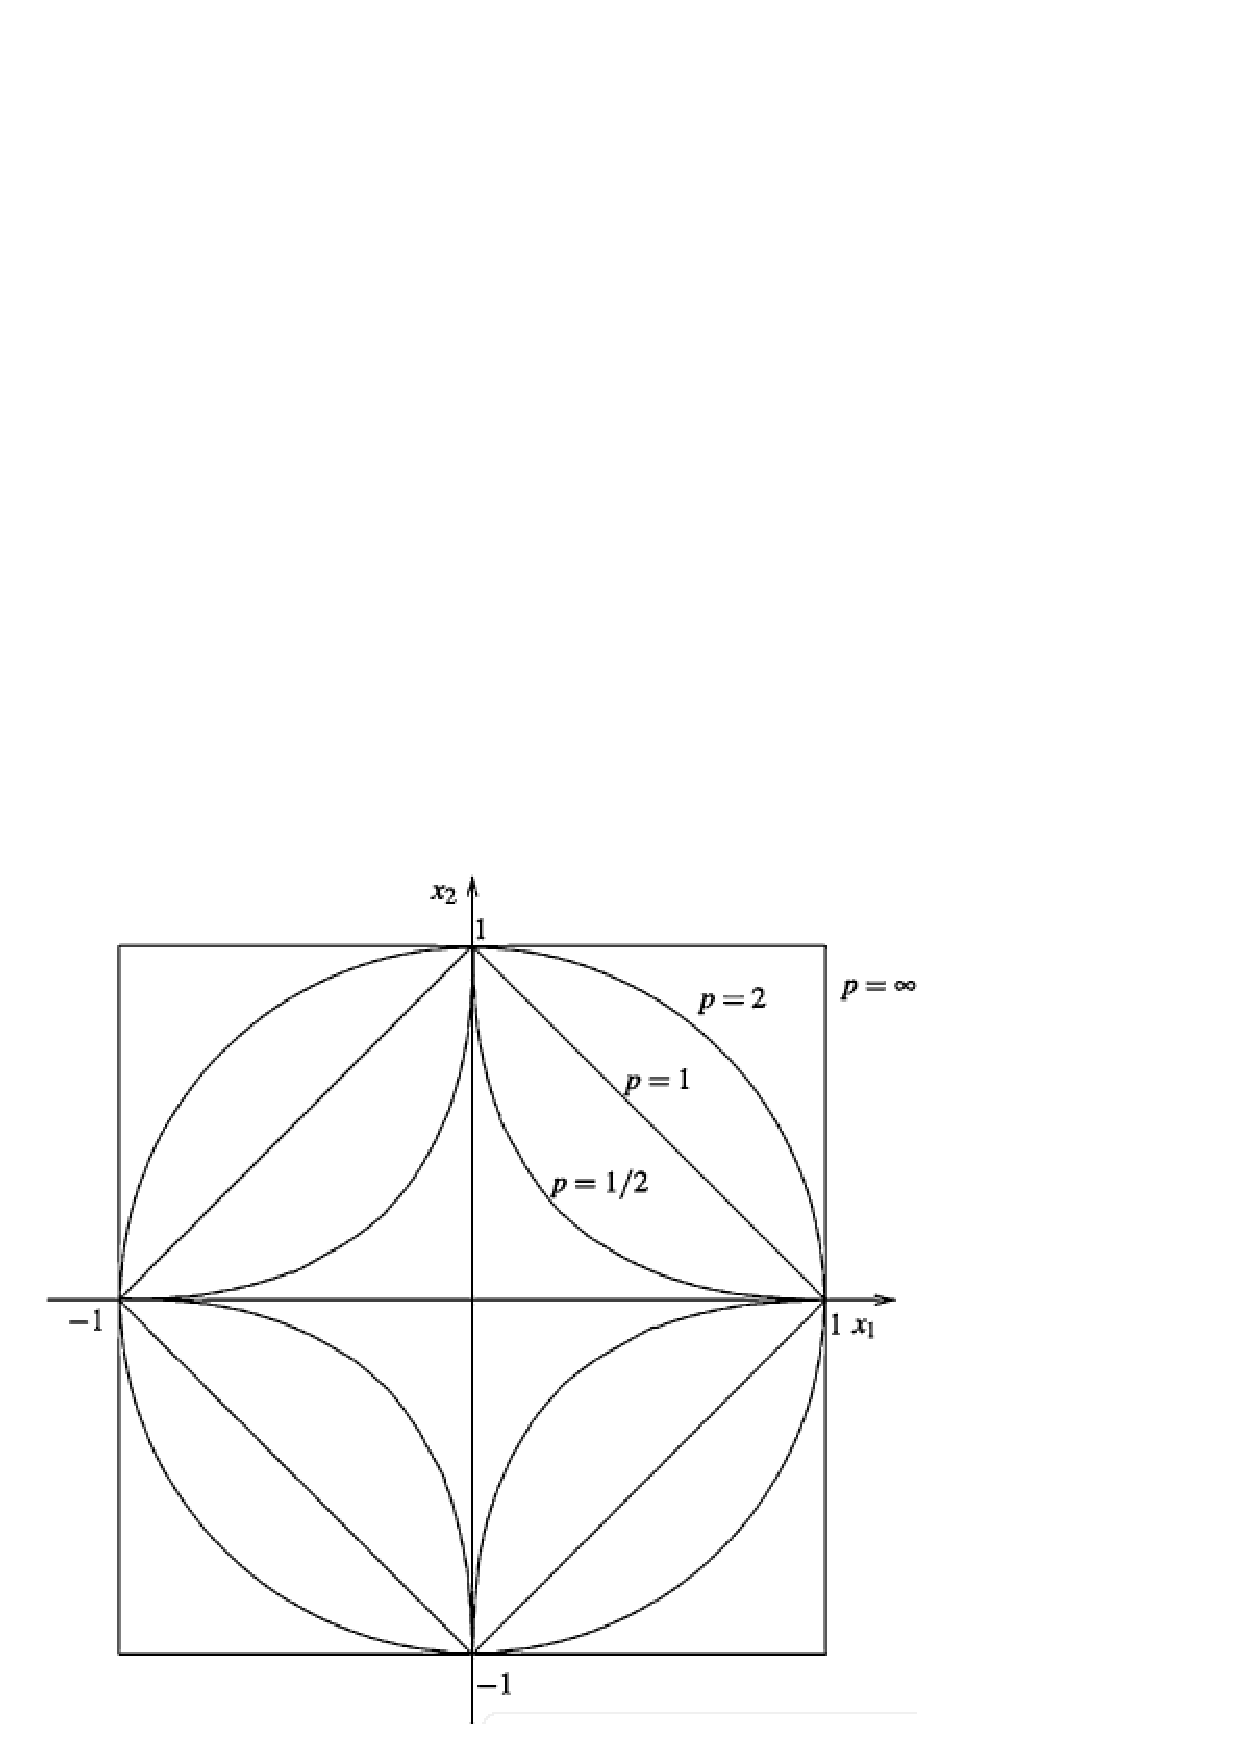
\includegraphics[scale=0.5]{Images/fig1.png}
\caption{پچ مایکرواستریپ با تغذیه ی کواکسیال}
\label{fig1}
\end{figure}
\begin{figure}
	\centering
	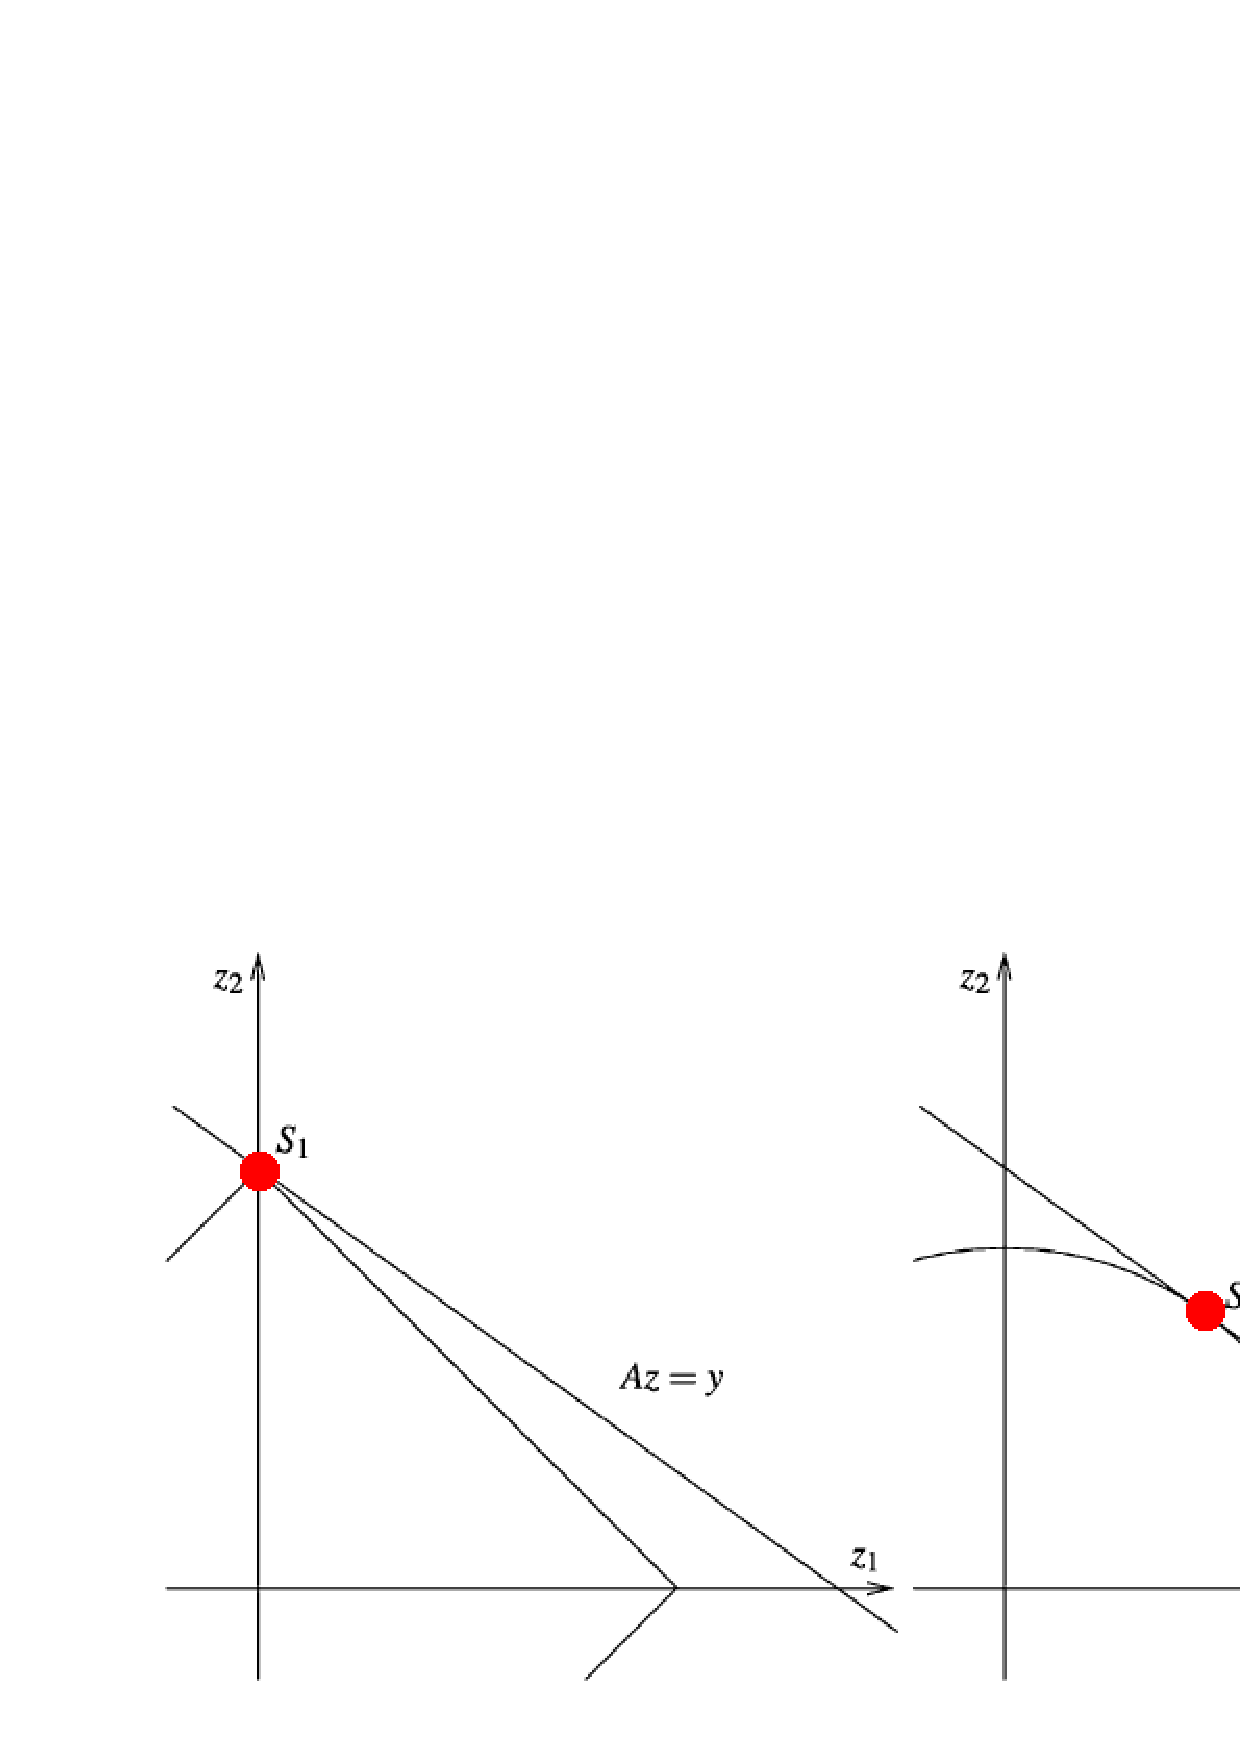
\includegraphics[scale=0.3]{Images/fig2.png}
	\caption{پچ مایکرواستریپ با تغذیه ی خط مایکرواستریپ}
	\label{fig2}
\end{figure}


از میان اشکال مختلف پَچ، انواع مربعی، مستطیلی به دلیل ویژگی‌های تشعشعی مطلوب بیشترین کاربرد را دارند.

\section{معایب آنتن مایکرواستریپ}
بازده پایین، توان پایین، قطبی‌شدگی خالص کم، عملکرد تطبیق ضعیف (فاکتور
$Q$
 بالاتر از ۱۰۰)، تأثیر تغذیه کاذب، و پهنای باند فرکانسی باریک (که در حد یک درصد و در نهایت چند درصد است) را می‌توان از معایب آنتن‌های مایکرواستریپ برشمارد.

البته راهکارهایی مانند افزایش ضخامت زیرلایه، می‌تواند بازده را تا ۹۰ درصد و پهنای باند را تا ۳۵ درصد افزایش دهد. البته با افزایش ضخامت زیرلایه، امواج سطحی
\LTRfootnote{Surface Wave}
 که مطلوب نیستند را نیز باید در نظر گرفت. امواج سطحی به علت تضعیف توان ارسالی مطلوب نیستند. امواج سطحی در زیرلایه انتقال می‌یابند و در ناپیوستگی‌ها و خمیدگی‌ها، مانند نقاط اتصال با صفحه زمین 
\LTRfootnote{Ground Plane}
 ظاهر خواهند شد که مشخصات آنتن (مانند الگوی تشعشع) را تغییر می‌دهد. امواج سطحی وقتی آنتن در یک حفره قرار می‌گیرد قابل صرف‌نظر است.


آنتن مایکرواستریپ خارج از ناحیه عملکرد، اثر الکترومغناطیسی زیادی در فرکانس‌های مشخص خواهد داشت. در سیستم‌های آرایه‌ای حتی در
\lr{VHF}\LTRfootnote{Very High Frequency}
 و
\lr{UHF}\LTRfootnote{Ultra High Frequency}
 بین پهنای باند و نرخ تطبیق، داد و ستد
\LTRfootnote{Trade-off}
  وجود دارد.


\section{انواع تغذیه}
\begin{figure}
	\centering
	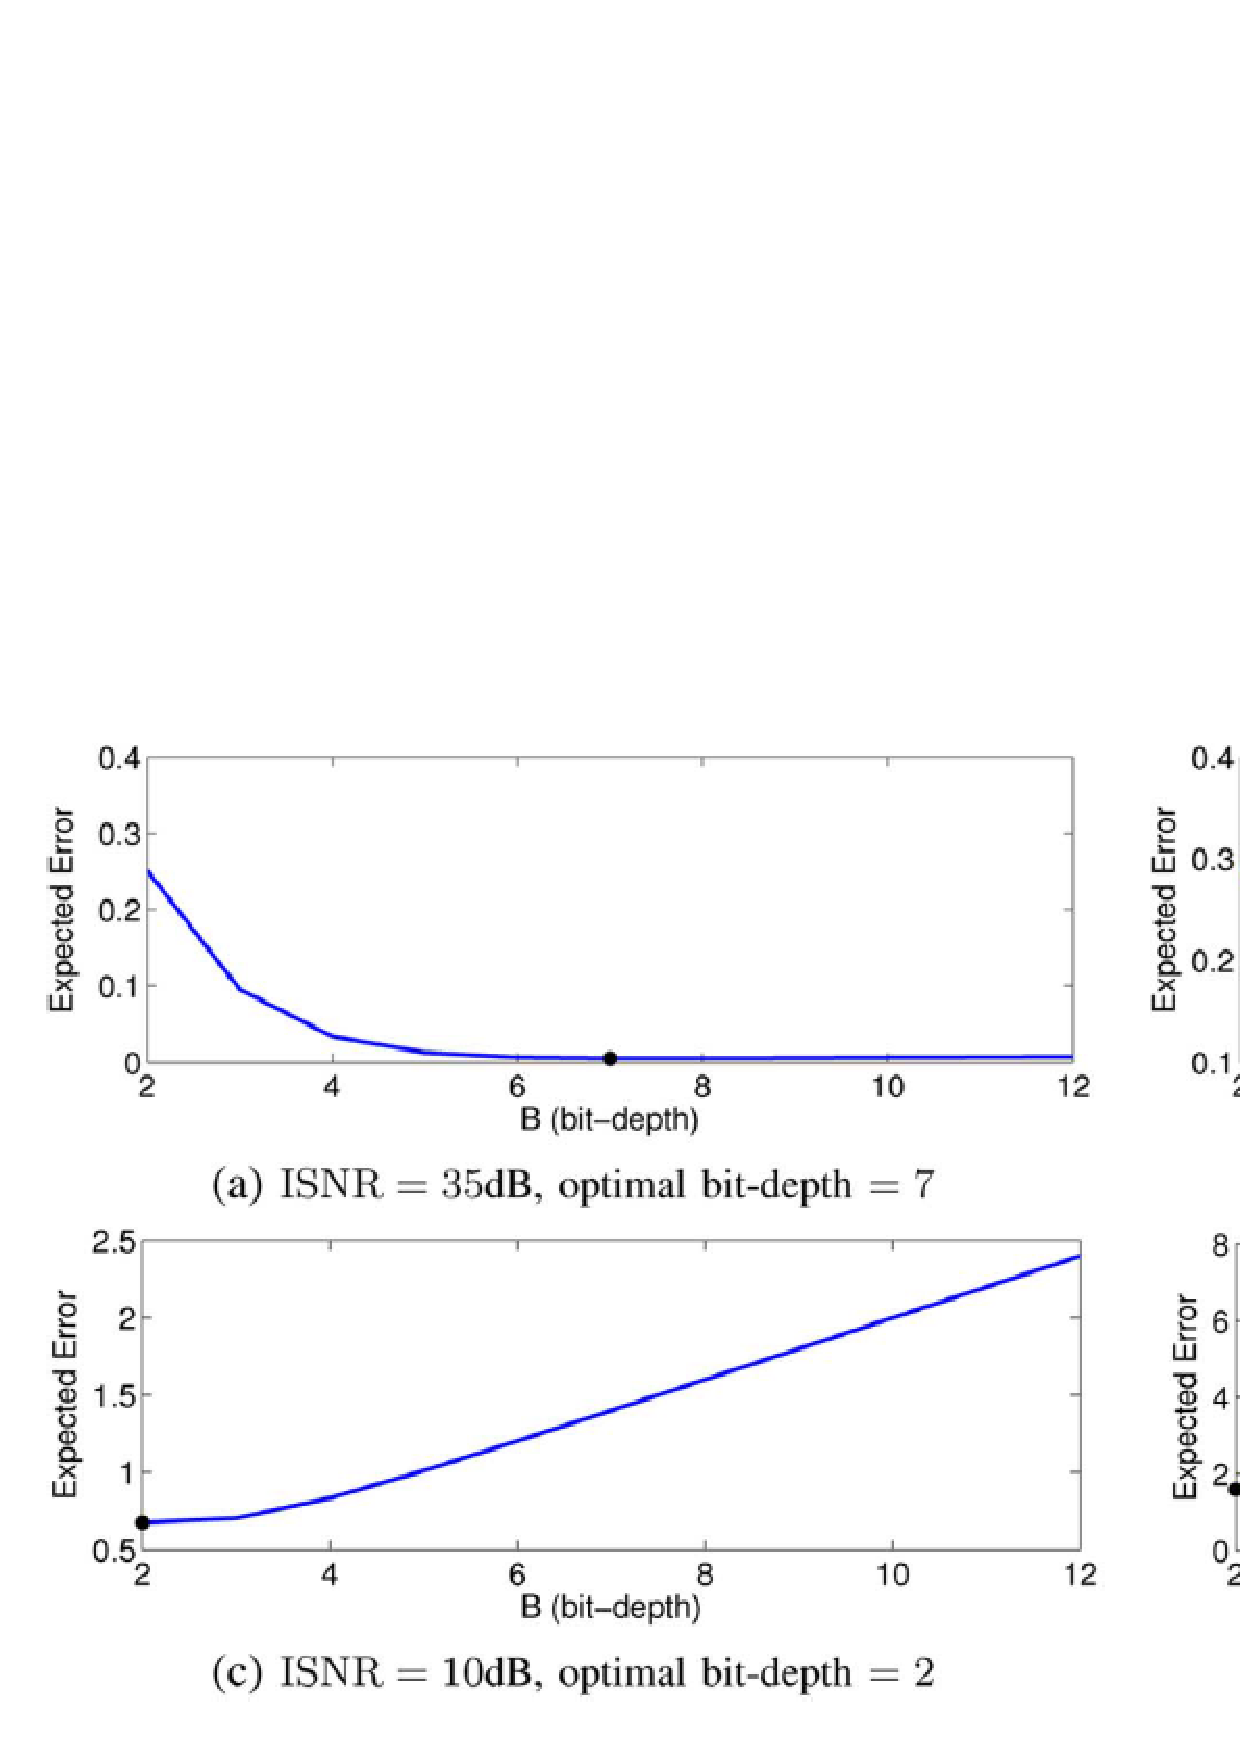
\includegraphics[scale=0.3]{Images/fig3.png}
	\caption{آنتن با تغذیه ی مایکرواستریپ}
	\label{fig3}
\end{figure}
روش‌های متعددی برای تغذیه آنتن‌های مایکرواستریپ وجود دارد که از جمله متداول‌ترین آن‌ها می‌توان به تغذیه توسط خط مایکرواستریپ
\LTRfootnote{Microstrip Line Feed}،
تغذیه کوپلینگ روزنه‌ای
\LTRfootnote{Aperture Coupling}،
 (شکل
\ref{fig4}
)
تغذیه کوپلینگ مجاورتی
\LTRfootnote{Proximity Coupling}
(شکل
\ref{fig5}
)
و تغذیه پروب کواکسیال
\LTRfootnote{Coaxial Probe Feed} 
 (شکل
\ref{fig6}
)
اشاره نمود.  



\subsection{آنتن با تغذیه ی کوپلینگ روزنه ای}
\begin{figure}
	\centering
	\includegraphics[scale=0.4]{Images/fig4.png}
	\caption{آنتن با تغذیه ی کوپلینگ روزنه ای}
	\label{fig4}
\end{figure}

\subsection{آنتن با تغذیه ی کوپلینگ مجاورتی}
\begin{figure}
	\centering
	\includegraphics[scale=0.7]{Images/fig5.png}
	\caption{آنتن با تغذیه ی کوپلینگ مجاورتی}
	\label{fig5}
\end{figure}

\subsection{آنتن با تغذیه ی کواکسیال}
در تغذیه آنتن‌های مایکرواستریپ از طریق کابل کواکسیال، هادی مرکزی کابل به پچ و شیلد خارجی کابل به صفحه زمین متصل می‌شود. این روش تغذیه به دلیل سادگی ساخت و امکان تطبیق آسان امپدانس، به طور گسترده‌ای مورد استفاده قرار می‌گیرد. با این حال، این نوع اتصال دارای پهنای باند محدود است و مدل‌سازی دقیق آن در شبیه‌سازی‌ها دشوار می‌باشد.(شکل
\ref{fig6})
\begin{figure}
	\centering
	\includegraphics[scale=0.3]{Images/fig6.png}
	\caption{آنتن با تغذیه ی کواکسیال}
	\label{fig6}
\end{figure}


\subsection{آنتن با پچ مستطیلی}
آنتن‌های با پچ مستطیلی به دلیل طراحی ساده، اندازه فشرده و عملکرد پایدار، به‌طور گسترده در سیستم‌های مخابراتی، ماهواره‌ای و راداری مورد استفاده قرار می‌گیرند. در این پژوهش، از روش تغذیه کواکسیال بهره گرفته شده است که در آن هادی مرکزی کابل مستقیماً به پچ و شیلد خارجی به صفحه زمین متصل می‌شود. این روش به دلیل سادگی ساخت، اتلاف پایین و قابلیت تطبیق امپدانس کارآمد، انتخاب شده است؛ هرچند که دارای محدودیت ذاتی در پهنای باند است.(شکل 
\ref{fig7})
\begin{figure}
	\centering
	\includegraphics[scale=0.9]{Images/fig7.jpg}
	\caption{آنتن با پچ مستطیلی}
	\label{fig7}
\end{figure}

در این پروژه، از روش تغذیه پروب کواکسیال استفاده شده است که دلیل انتخاب آن، سادگی ساخت، اتلاف کم و قابلیت اطمینان بالا در کاربردهای عملی است. در ادامه، به بررسی دقیق‌تر اصول کاری و ملاحظات طراحی این روش پرداخته خواهد شد.


\section{اثر لبه}

به دلیل محدودیت ابعاد پچ در راستای طول و عرض، میدان‌های الکترومغناطیسی از لبه‌های پچ به بیرون انتشار می‌یابند که این پدیده تحت عنوان اثر لبه‌ای
\LTRfootnote{Fringing Effect}
شناخته می‌شود
\cite{chahar}.
همانطور که در شکل 
\ref{fig8}
نشان داده شده است
این اثر منجر به گسترش میدان‌ها در خارج از مرزهای فیزیکی پچ می‌گردد.

\begin{figure}
	\centering
	\includegraphics[scale=0.3]{Images/fig8.png}
	\caption{اثر لبه در پچ مایکرواستریپ}
	\label{fig8}
\end{figure}

میزان تراوش میدان از لبه‌ها تابعی از ابعاد هندسی پچ (طول
$L$
 و عرض
$W$)
 و همچنین ویژگی‌های زیرلایه از جمله ارتفاع (
$h$)
 و ثابت دی‌الکتریک (
 $\varepsilon_r$)
 است. برای صفحه اصلی
 $E$،
  این اثر به طور خاص به نسبت
$L$
  و
$\varepsilon_r$
 وابسته می‌باشد.


همانطور که در شکل بالا مشاهده می‌شود، بخش عمده‌ای از خطوط میدان در داخل زیرلایه متمرکز شده‌اند، در حالی که بخشی از آن‌ها به محیط اطراف (هوا) نفوذ می‌کنند. در شرایطی که
$ \frac{W}{h} \gg 1$
 باشد، تراکم خطوط میدان عمدتاً درون زیرلایه رخ می‌دهد. اثر لبه‌ای سبب می‌شود که طول الکتریکی پچ بزرگ‌تر از ابعاد فیزیکی آن به نظر رسد. از آنجایی که بخشی از میدان در هوا و بخشی دیگر در زیرلایه انتشار می‌یابد، یک ثابت دی‌الکتریک مؤثر(
$\varepsilon_{e}$)
 تعریف می‌شود تا تأثیر هر دو محیط به صورت همزمان در محاسبات در نظر گرفته شود. این کمیت به صورت تحلیلی و بر اساس پارامترهای ساختاری آنتن محاسبه شده و نقش اساسی در تعیین دقیق فرکانس تشدید و سایر پارامترهای الکتریکی آنتن ایفا می‌کند.


برای تعریف ثابت دی‌الکتریک موثر، فرض می‌کنیم لایه رسانا با ابعاد اصلی خود (مطابق شکل فوق) در میان زیرلایه قرار گرفته است. ثابت دی‌الکتریکی‌ای که در این حالت، همان مشخصه انتشار حالت قبل را از خود نشان دهد را ثابت دی‌الکتریک موثر(
$\varepsilon_{e}$)
می‌نامند.


اگر ثابت دی‌الکتریک زیرلایه(
$\varepsilon_r$)
بسیار بزرگ باشد، ثابت موثر(
$\varepsilon_{e}$)
به ثابت زیرلایه(
$\varepsilon_{r}$)
نزدیک‌تر است. به علاوه، ثابت موثر تابعی از فرکانس نیز می‌باشد. شکل 
\ref{fig9}
 رابطه بین ثابت موثر دی‌الکتریک و فرکانس را برای سه زیرلایه متفاوت نشان می‌دهد.

\begin{figure}
	\centering
	\includegraphics[scale=0.3]{Images/fig9.png}
	\caption{رابطه ی بین ثابت موثر دی الکتریک و فرکانس}
	\label{fig9}
\end{figure}

ثابت موثر دی الکتریک از معادلات 
\ref{eq:eq2}
و
\ref{eq:eq3}
بدست می آید:

\begin{align}
 	\label{eq:eq2}
    \frac{W}{H} < 1	\qquad  \varepsilon_e = \frac{\varepsilon_r+1}{2} + \frac{\varepsilon_r-1}{2} \left[ \left(1+12\frac{H}{W}\right)^{-1/2} + 0.04 \left(1-\frac{W}{H}\right)^2 \right]
\end{align}


\begin{align}
	\label{eq:eq3}
    \frac{W}{H} \geq 1 \qquad \varepsilon_e = \frac{\varepsilon_r+1}{2} + \frac{\varepsilon_r-1}{2} \left(1+12\frac{H}{W}\right)^{-1/2} 
\end{align}


\section{طول موثر، فرکانس تشدید و پهنای باند موثر}
به دلیل اثر حاشیه‌ای
\LTRfootnote{Fringing Effect}،
 طول الکتریکی پَچ به اندازه
$ \delta L$
 افزایش می‌یابد. این افزایش تابعی از ثابت دی‌الکتریک مؤثر(
 $\varepsilon_{e}$)
 و نسبت عرض به ارتفاع
 $W/h$
  زیرلایه است که از رابطه تجربی 
\eqref{eq:eq4}
   محاسبه می‌شود.
\begin{align}
	\label{eq:eq4}
	\frac{\Delta L}{h} = 0.412 \frac{(\varepsilon_{e}+0.3)\left(\frac{W}{h}+0.264\right)}{(\varepsilon_{e}-0.258)\left(\frac{W}{h}+0.8\right)}
\end{align}


\begin{figure}
	\centering
	\includegraphics[scale=0.3]{Images/fig10.png}
	\caption{رابطه ی بین ثابت موثر دی الکتریک و فرکانس}
	\label{fig10}
\end{figure}

\begin{figure}
	\centering
	\includegraphics[scale=0.3]{Images/fig11.png}
	\caption{طول های فیزیکی و موثر پچ مایکرواستریپ مستطیلی}
	\label{fig11}
\end{figure}

با در نظر گیری این اثر، طول مؤثر پَچ(
$L_{e}$)
برای محاسبه فرکانس تشدید به صورت 
\eqref{eq:eq5}
 تعریف می‌شود.که در آن 
 $L$
  طول فیزیکی پَچ است.
\begin{align}
	\label{eq:eq5}
	L_{e} = L + 2\delta L
\end{align}

برای مد غالب
$TM_{010}$
فرکانس تشدید به صورت 
\eqref{eq:eq6}
است.
\begin{align}
	\label{eq:eq6}
	(f_r)_{010} = \frac{1}{2L\sqrt{\varepsilon_r}\sqrt{\mu_0\varepsilon_0}} = \frac{v_0}{2L\sqrt{\varepsilon_r}}
\end{align}
$v_0$
سرعت نور در فضای آزاد است.

با در نظرگیری اثر حاشیه‌ای، محاسبه فرکانس تشدید نیازمند اصلاح طول پچ و استفاده از ثابت دی‌الکتریک مؤثر است. فرکانس تشدید برای حالت پایه
$TM_{10}$
 به صورت
\eqref{eq:eq7}
  محاسبه می‌شود.
\begin{align}
	\label{eq:eq7}
	(f_r)_{010} = \frac{1}{2L_{e}\sqrt{\varepsilon_{e}}\sqrt{\mu_0\varepsilon_0}} = \frac{c}{2(L+2\Delta L)\sqrt{\varepsilon_{e}}}
\end{align}

ضریب تراوش
$q$
 به عنوان نسبت فرکانس تشدید واقعی به فرکانس تشدید بدون در نظرگیری اثر حاشیه‌ای به صورت
\eqref{eq:eq8}
  تعریف می‌شود.
\begin{align}
	\label{eq:eq7}
	q = \frac{(f_r)_{\text{actual}}}{(f_r)_{\text{without fringing}}}
\end{align}

با افزایش ارتفاع زیرلایه (
$h$)،
 اثر حاشیه‌ای تشدید شده و موجب افزایش
 $\Delta L$
  و در نتیجه کاهش فرکانس تشدید می‌گردد. این پدیده به‌طور مستقیم بر عملکرد آنتن تأثیر گذاشته و طراحی را به سمت استفاده از مدل‌های دقیق‌تر برای پیش‌بینی رفتار آنتن سوق می‌دهد.












\newpage 
\chapter{آنتن آرایه ای ، تزویج ( کوپلینگ ) و راه های کاهش آن}
\label{ch:2}
\section{مقدمه}
پس از آشنایی با اصول طراحی و تحلیل آنتن‌های مایکرواستریپ تکی، در این فصل به بررسی آرایه‌های آنتن و چالش‌های مرتبط با تزویج متقابل
\LTRfootnote{Coupling}
 بین المان‌های آرایه پرداخته می‌شود. هدف اصلی، تبیین مکانیزم‌های تزویج و ارائه راه‌کارهای عملی برای کاهش اثرات نامطلوب آن در عملکرد آرایه است.
 
\section{آرایه ها و شبکه ی تغذیه}
آرایهٔ آنتنی به مجموعه‌ای از چندین المان تشعشعی گفته می‌شود که به صورت منظم یا نامنظم در کنار یکدیگر قرار گرفته و با تغذیهٔ مناسب، الگوی تشعشعی دلخواه ایجاد می‌کنند. آرایه‌ها معمولاً از ترکیب آنتن‌های ساده‌ای مانند پچ، دیپل یا شکاف ساخته می‌شوند و با تنظیم دامنه و فاز جریان تغذیهٔ هر المان، می‌توان شکل پرتو را کنترل و در جهات مختلف هدایت کرد.


آرایه‌ها کاربردپذیری بالایی دارند و برای تولید الگوهای تشعشعی مورد نظر که با یک المان منفرد قابل دستیابی نیستند، استفاده می‌شوند. به علاوه، برای چرخاندن پرتو یک سیستم آنتن، افزایش سمت‌گرایی
\LTRfootnote{Directivity}
 و انجام کارهایی که با المان‌های تکی دشوار است، به‌کار گرفته می‌شوند. به همین دلیل، آرایه‌ها نقش کلیدی در رادارها، سیستم‌های مخابرات ماهواره‌ای،
 \lr{5G}
  و سامانه‌های
  \lr{MIMO}
   ایفا می‌کنند.
   
   
   آرایه ها به دو صورت میتوانند تغذیه شوند:‌ تغذیه ی سری و موازی. البته به صورت ترکیبی هم ممکن است.
   

\begin{figure}[t]
	\centering
	\begin{subfigure}{0.3\textwidth} % width of left subfigure
		\includegraphics[scale=0.2]{Images/fig12.png}
		\caption{تغذیه سری} % subcaption
		\label{fig12}
	\end{subfigure}
	\vspace{1em} % here you can insert horizontal or vertical space
	\begin{subfigure}{0.3\textwidth} % width of right subfigure
		\includegraphics[scale=0.2]{Images/fig13.png}
		\caption{تغذیه موازی} % subcaption
		\label{fig13}
	\end{subfigure}
		\vspace{1em} % here you can insert horizontal or vertical space
	\begin{subfigure}{0.3\textwidth} % width of right subfigure
		\includegraphics[scale=0.2]{Images/fig14.png}
		\caption{تغذیه سری موازی} % subcaption
		\label{fig14}
	\end{subfigure}
	\caption{تغذیه آرایه ها}
\end{figure}


در این روش که برای تقسیم توان به توان‌های
$ 2^n$
 (یعنی ۲، ۴، ۸، ۱۶ و ...) استفاده می‌شود، تقسیم توان با استفاده از خطوط تغذیه باریک‌شونده
\LTRfootnote{Tapered Lines}
 مطابق شکل زیر انجام می‌شود تا امپدانس المان‌های پَچ (معمولاً ۱۰۰ اهم) را به امپدانس ورودی استاندارد (۵۰ اهم) تطبیق دهد.



\begin{figure}
	\centering
	\includegraphics[scale=0.3]{Images/fig15.png}
	\caption{خطوط باریک شونده}
	\label{fig15}
\end{figure}

به علاوه میتوان با مبدل های امپدانس ربع طول موج هم این کار را انجام داد:
\begin{figure}
	\centering
	\includegraphics[scale=0.4]{Images/fig16.png}
	\caption{مبدل یک چهارم طول موج}
	\label{fig16}
\end{figure}

آرایه‌های تغذیه سری را می‌توان به راحتی با استفاده از مدل چاپی نوری برای المان‌های تشعشعی و شبکه تغذیه ساخت. البته این روش به آرایه با پرتو ثابت یا آرایه‌هایی که با تغییر فرکانس اسکن می‌شوند محدود می‌شود، ولی می‌توان از این تکنیک برای آرایه‌های خطی صفحه‌ای با پلاریزاسیون تکی یا دوگانه استفاده کرد. همچنین هرگونه تغییر در یکی از المان‌ها یا خطوط تغذیه، عملکرد بقیه را تحت تأثیر قرار می‌دهد. بنابراین در یک طراحی، در نظر گرفتن این اثرات و سایر اثرات مانند تلفیق متقابل و بازتابش‌های داخلی مهم است.


آرایه‌های تغذیه مشارکتی، متداول و دارای کاربردهای متنوعی هستند. با این روش، طراح کنترل بیشتری روی تغذیه هر المان (دامنه و فاز) دارد و این روش برای آرایه‌های فاز اسکن‌کننده، آرایه‌های چندپرتوئی یا آرایه‌های با پرتو شکل‌داده‌شده، ایده‌آل است. فاز هر المان را با استفاده از شیفت‌دهنده‌ها می‌توان کنترل کرد و دامنه را با استفاده از تقویت‌کننده‌ها و تضعیف‌کننده‌ها می‌توان تحت کنترل قرار داد.


نکته قابل توجه این است که چه در تغذیه سری و چه در مشارکتی، تشعشع از خط تغذیه قابل ملاحظه و مهم است که پلاریزاسیون را متقاطع و سطح لوب کناری آرایه را افزایش می‌دهد. که هر دو را می‌توان با جداسازی شبکه تغذیه از صفحه تشعشع‌کننده آرایه بهبود بخشید که این کار را می‌توان با استفاده از تغذیه‌های پروبی یا تغذیه روزنه‌ای انجام داد.


\section{تزویج}
یکی از مسائل مهم در طراحی آرایه‌های آنتنی، تزویج متقابل میان عناصر آرایه است. هنگامی که المان‌ها در فاصله‌ای کمتر از چندین طول‌موج قرار گیرند، میدان‌های الکترومغناطیسی هر المان بر سایر المان‌ها اثر می‌گذارد. این پدیده باعث می‌شود که جریان‌های القاشده روی المان‌های مجاور تغییر کنند و در نتیجه امپدانس ورودی، بهره و الگوی تابش کل آرایه دچار تغییر شود.


این تزویج باعث بوجود آمدن تغییرات زیر میشود : 

\begin{itemize}
	\item{
	انحراف امپدانس ورودی از مقدار طراحی شده
	} 
	\item{
	کاهش بهره و بازدهی آرایه
	}
	\item{
	تغییر در الگوی تشعشعی (افزایش
	\lr{sidelobe}
	ها).
	}
	\item{
	محدودیت پهنای باند عملیاتی.
	}
\end{itemize}

دو نوع چیدمان برای پَچ‌های میکرواستریپ وجود دارد: یکی در راستای محور
$ y$
 و دیگری در راستای محور
 $ x$
 (شکل
 \ref{fig17}).

هدف از میدانی که با تنظیم خطوط تغذیه در طول
$ y$
 قرار داده می‌شوند، این است که میدان‌های الکتریکی تشعشعی در تشدید در طول
 $ L$،
  پلاریزاسیون خطی ایجاد کند. 


این بدین معنی است که میدان‌های الکتریکی تشعشع‌یافته در طول
$ y$
 بیشتر پلاریزه می‌شوند و این نیز به معنای تزویج بیشتر در این وضعیت است. در نتیجه، این وضعیت نشان می‌دهد که چیدمان پَچ در طول محور
 $ x$،
  تزویج متقابل
\LTRfootnote{Mutual Coupling}
 را کاهش می‌دهد.
 
\begin{figure}
	\centering
	\includegraphics[scale=1.5]{Images/fig17.jpg}
	\caption{قرار گیری پچ ها در راستای 
		$x$ 
		و 
		$y$}
	\label{fig17}
\end{figure}

میتوان نشان داد که تزویج بین دو پچ تابع مکان یکی نسبت به دیگریست. برای این امر به مقاله ی
\cite{carver1981microstrip}
 استناد میکنیم. در این مقاله ثابت شده که با افزایش فاصله بین دو پچ ، تزویج متقابل نیز کاهش میابد. 

\begin{figure}
	\centering
	\includegraphics[scale=1.5]{Images/fig18.jpg}
	\caption{آرایش صفحه های E و H آنتن های مایکرواستریپ}
	\label{fig18}
\end{figure}

در نمودار 
\ref{fig19}
 تغییرات تزویج متقابل بین دو پچ در فواصل مختلف در دو آرایش E و H از مقاله ی 
 \cite{carver1981microstrip}
  نمایش داده میشود. 

\begin{figure}
	\centering
	\includegraphics[scale=1]{Images/fig19.jpg}
	\caption{نمودار تزویج متقابل بین دو پچ در آرایش E و H}
	\label{fig19}
\end{figure}

در شکل فوق ابعاد آنتن به صورت زیر میباشد:
\begin{align}
	\label{eq:eq8}
	W = 10.57 \text{cm}, L = 6.55 \text{cm}, h = 0.1588 \text{cm}, \varepsilon_r = 2.55, f_r = 1.410 \text{MHz}
\end{align}

ابعاد
$ L$
 و
 $ W$
  از فرمول های 
  \ref{eq:eq9}
   تبعیت میکنند:
\begin{align}
	\label{eq:eq9}
	W = \frac{c}{2f_r\sqrt{\frac{\varepsilon_r+1}{2}}}
\end{align}
که در آن:
\begin{itemize}
	\item{$W$:
	عرض پچ(بر حسب متر)
	}
	\item{$c$:
	سرعت نور در خلاء
	}
	\item{$f_r$:
	فرکانس رزونانس (بر حسب هرتز)
	}
	\item{$\varepsilon_{r}$:
	ثابت دی الکتریک نسبی زیرلایه
	}
\end{itemize}


\begin{align}
	\label{eq:eq10}
	\varepsilon_{\text{eff}} = \frac{\varepsilon_R+1}{2} + \frac{\varepsilon_R-1}{2}\left[\frac{1}{\sqrt{1+12\left(\frac{h}{W}\right)}}\right]
\end{align}

\begin{align}
	\label{eq:eq11}
	\text{Length} = \frac{c}{2f_0\sqrt{\varepsilon_{e}}} - \left(2 \times \left[0.412h\frac{(\varepsilon_{e}+0.3)\left(\frac{W}{h}+0.264\right)}{(\varepsilon_{e}-0.258)\left(\frac{W}{h}+0.8\right)}\right]\right)
\end{align}

که با جایگذاری به تقریبا به همین اعداد میرسیم.


در تزویج بین دو پَچ مستطیلی، اگر المان‌ها هم‌راستا در صفحه E باشند، این آرایش، آرایش صفحه E نامیده می‌شود و اگر هم‌راستا در صفحه H باشند، این آرایش، آرایش صفحه H نام خواهد گرفت.

در آرایش صفحه E، معمولاً برای فواصل بسیار کوچک(
$s < 0.10\lambda$)،
 بیشترین تزویج را نشان می‌دهد، در حالی که در آرایش صفحه H، معمولاً برای فواصل بزرگ(
 $s > 0.10\lambda$)،
  کمترین تزویج را نشان می‌دهد. فاصله‌ای که در آن تزویج یک صفحه از دیگری پیشی می‌گیرد، به خواص الکتریکی و ابعاد هندسی آنتن مایکرواستریپ بستگی دارد.

به طور کلی، تزویج متقابل بیشتر به میدان‌هایی که در امتداد فصل‌مشترک هوا با دی‌الکتریک وجود دارند مربوط میشود. این میدان ها میتوانند به امواج فضایی(با تغییرات شعاع
$1/\rho$)
امواج مرتبه بالاتر(با تغییرات شعاع
$1/\rho^2$)
امواج سطحی(با تغییرات شعاع
$1/\rho^{\frac{1}{2}}$)
وامواج نشطی(با تغییرات شعاع
$\exp{-\lambda_{p}/\rho^{\dfrac{1}{2}}}$)
تجزیه شوند. به دلیل تغییرات شعاعی کروی، امواج فضایی و مرتبه بالاتر برای فواصل کوچک و امواج سطحی برای فواصل بزرگ غالب می‌شوند.


امواج سطحی که داخل دی‌الکتریک وجود دارد، در آن منتشر می‌شود و تحریک آن‌ها تابعی از ضخامت دی‌الکتریک است. برای یک پَچ مستطیلی، میدان‌ها در جهت انتشار در امتداد صفحه E از نوع TM و در امتداد صفحه H از نوع TE هستند. در آرایش صفحه E، همانطور که در شکل فوق نشان داده شده، المان‌ها در راستای صفحه E قرار دارند و در فاصله بین المان‌ها میدان از نوع TM است. یک تحریک موج سطحی قوی‌تر بین المان‌ها وجود دارد و تزویج بزرگتر است. اما در صفحه H این گونه نیست و تحریک موج سطحی قوی وجود ندارد و تزویج کمی وجود دارد. با افزایش ضخامت زیرلایه که باعث تحریک موج سطحی TE مرتبه بالاتر می‌شود، این تزویج تغییر می‌کند.



از آنجا که این مقاله پایه ی پروژه ی ماست ، عینا همین مقاله را در نرم افزار HFSS شبیه سازی کردم و نتایج به در شکل های 
\ref{fig20}
،
\ref{fig21}
،
\ref{fig22}
و
\ref{fig23}
نشان داده شده است.

 

\begin{figure}
	\includegraphics[scale=0.5]{Images/fig20.jpg}
	\caption{قرار گیری پچ ها در آرایش H-plain}
	\label{fig20}
\end{figure}
\begin{figure}
	\includegraphics[scale=0.5]{Images/fig21.jpg}
	\caption{نمودار \lr{Return loss} در آرایش H-plain }
	\label{fig21}
\end{figure}

\begin{figure}
	\includegraphics[scale=0.5]{Images/fig22.jpg}
	\caption{قرار گیری پچ ها در آرایش E-plain}
	\label{fig22}
\end{figure}
\begin{figure}
	\includegraphics[scale=0.5]{Images/fig23.jpg}
	\caption{نمودار \lr{Return loss} در آرایش E-plain }
	\label{fig23}
\end{figure}

\begin{figure}
	\centering
	\begin{subfigure}{0.5\textwidth} % width of left subfigure
		\includegraphics[scale=0.25]{Images/H-plane.png}
		\caption{H-plane} % subcaption
		\label{fig24}
	\end{subfigure}
	\vspace{1em} % here you can insert horizontal or vertical space
	\begin{subfigure}{0.5\textwidth} % width of right subfigure
		\includegraphics[scale=0.25]{Images/E-plane.png}
		\caption{E-plane} % subcaption
		\label{fig25}
	\end{subfigure}
	\caption{نمودار مقایسه ی تزویج متقابل مقاله ی کارور و شبیه سازی HFSS در آرایش های E-Plain و H-Plain }
\end{figure}


در نتیجه با تقریب مناسبی ثابت شد که با افزایش فاصله در هر دو آرایش E و H ، مقدار تزویج متقابل کاهش میابد.

\section{راه های کاهش تزویج متقابل}
 در مقاله ی آقای کارور ثابت شد که با افزایش فاصله ، تزویج متقابل کاهش پیدا میکند این روش ساده ترین راه برای کاهش تزویج متقابل بدون تغییر پیچیده در ساختار است اما موجب افزایش ابعاد کل  آرایه  مي شود و در کاربردهایی که فضای محدود دارند (مانند آنتن های ماهوارەای یا سیستم های
 \lr{5G}
  فشرده) مناسب نیست. 
برای کاهش پدیدۀ تزویج متقابل میان المان های آرایەهای آنتن، روش های متعددی وجود دارد. انتخاب روش مناسب وابسته به محدودیت های طراحی (ابعاد، باند فرکانسی ، بهره، پیچیدگی ساخت) است. در ادامه ی این گزارش مرسوم ترین روش ها بررسی شده است.

\subsection{	استفاده از ساختارهای زمین ایزوله}
	در  روش  ساختارهای زمین ایزوله
	\LTRfootnote{Isolation Structures}
	 با ایجاد شیارها یا شکاف‌هایی در صفحه زمین، مسیر جریان‌های سطحی محدود می‌شود. این کار باعث کاهش انتقال انرژی ناخواسته میان المان‌ها می‌شود(
	\cite{alibakhshikenari2018antenna}, \cite{emadeddin2017high})
	
	
			مزایا:
	\begin{itemize}
		\item{
	پیاده‌سازی ساده با تغییر در صفحه زمین.
		}
		\item{
امکان استفاده در فرکانس‌های مختلف بدون تغییر اساسی در طراحی.
		}
	\end{itemize}


معایب:
\begin{itemize}
	\item{
	می‌تواند روی امپدانس ورودی و تطبیق اثر منفی بگذارد.
	}
	\item{
	کاهش بهره یا تغییر در الگوی تابش محتمل است.
	}
\end{itemize}


\subsection{
	به‌کارگیری متامواد یا ساختارهای دوره‌ای
}
		متامواد و ساختارهای دوره‌ای الکترومغناطیسی
	\LTRfootnote{EBG/Metasurface}
	 می‌توانند با ایجاد باند توقف امواج سطحی، از انتشار انرژی ناخواسته جلوگیری کنند. در نتیجه، کوپلینگ میان آنتن‌های مجاور به طور قابل توجهی کاهش می‌یابد.(
	\cite{ledimo2022design},\cite{yang2003microstrip},\cite{rahim2008electromagnetic},\cite{tang2020metasurface})
	
	
			مزایا:
	\begin{itemize}
		\item{
		ایجاد باند توقف امواج سطحی و کاهش شدید کوپلینگ.	
		}
		\item{
			بهبود بهره و راندمان تابشی.
		}
		\item {
		کنترل لوب‌های جانبی در الگوی تشعشعی.
		}
	\end{itemize}
	معایب:
	\begin{itemize}
	\item{
طراحی و شبیه‌سازی پیچیده‌تر نسبت به سایر روش‌ها.
	}
	\item{
نیاز به ابعاد سلولی دقیق متناسب با 
$\lambda_0$.
	}
	\item {
حساسیت بالا به خطاهای ساخت.
	}
\end{itemize}	

\subsection{
	استفاده از ساختارهای  DGS
}
در روش
DGS\LTRfootnote{Defected Ground Structure}
 با ایجاد نقص‌های مهندسی‌شده (مانند شکاف‌های دمبل‌شکل یا U شکل) در صفحه زمین، مشخصات امپدانسی تغییر کرده و امواج سطحی تضعیف می‌شوند. DGS را می‌توان به‌صورت مدار معادل LC مدل کرد.(
\cite{hajilou2012mutual},\cite{ibrahim2014compact})


			مزایا:
	\begin{itemize}
		\item{
کاهش مؤثر کوپلینگ متقابل.
		}
		\item{
امکان کنترل پاسخ فرکانسی با تغییر ابعاد.
		}
		\item {
		قابلیت کوچک‌سازی آنتن یا ایجاد باند توقف باریک.
		}
	\end{itemize}

معایب:
\begin{itemize}
	\item {
		احتمال ایجاد تشعشع ناخواسته از صفحه زمین.
	}
	\item {
	افزایش حساسیت به خطای ساخت.
	}
	\item {
	در برخی موارد کاهش پهنای باند کاری.
	}
\end{itemize}

\subsection{
	طراحی بهینهٔ پیکربندی آرایه
}
با بهره‌گیری از الگوریتم‌های بهینه‌سازی هوشمند (مانند الگوریتم ژنتیک، PSO و غیره)، می‌توان مکان و فاصله‌ی عناصر آرایه را طوری انتخاب کرد که کوپلینگ کاهش یابد.(
\cite{ghadimi2020systematic})


مزایا:
\begin{itemize}
	\item {
		امکان دستیابی به طراحی فشرده با حداقل کوپلینگ.
	}
	\item {
	بدون نیاز به تغییر اساسی در زیرلایه یا صفحه زمین.
	}
\end{itemize}
معایب:
\begin{itemize}
	\item {
	زمان‌بر و نیازمند محاسبات سنگین.
	}
	\item{
	نتایج به شدت وابسته به الگوریتم انتخابی و قیود طراحی هستند.
	}
\end{itemize}


\section*{\textsf{جدول مقایسه روش‌های کاهش کوپلینگ}}

\begin{table}[h!]
\centering
\scriptsize
\renewcommand{\arraystretch}{1.3}
\begin{tabular}{|>{\RaggedLeft\arraybackslash}p{2cm}|>{\arraybackslash}p{2.2cm}|>{\centering\arraybackslash}p{1.3cm}|>{\centering\arraybackslash}p{1.5cm}|>{\arraybackslash}p{2.8cm}|>{\arraybackslash}p{2.8cm}|}
\hline
\textbf{منبع} & \textbf{روش کاهش کوپلینگ} & \textbf{میزان کاهش کوپلینگ (dB)} & \textbf{فاصله بین المان‌ها} & \textbf{مزایا} & \textbf{معایب} \\
\hline
\cite{hajilou2012mutual} & ساختار زمین خراشیده (DGS) & $23$ & $0.25\lambda_0$ & کاهش قابل توجه کوپلینگ، ساختار فشرده و ساده & احتمال تغییر الگوی تشعشعی، محدودیت پهنای باند \\
\hline
\cite{ghadimi2020systematic} & بهینه‌سازی دودویی المان پارازیتی & $24$ & نامشخص & کاهش شدید کوپلینگ، حفظ الگوی تشعشعی و تطابق امپدانس، عدم نیاز به تغییر صفحه زمین & پیچیدگی محاسباتی بالا، وابستگی به الگوریتم بهینه‌سازی \\
\hline
\cite{yang2003microstrip} & ساختار باند ممنوعه الکترومغناطیسی (EBG) & $8$ & $0.75\lambda_0$ & سرکوب موج سطحی، بهبود عملکرد آرایه & افزایش حجم ساختار، طراحی نسبتاً پیچیده \\
\hline
\cite{tang2020metasurface} & ابرسطح متامتریال (Metasurface) & $8-25$ & $0.43\lambda_0$ & کاهش کوپلینگ در آرایه‌های بزرگ، بهبود پهنای باند و الگوی تشعشعی & افزایش ارتفاع و حجم آنتن، پیچیدگی ساخت \\
\hline
\cite{emadeddin2017high} & ترکیب اسلات و نوارهای پارازیتی & $41$ & $0.28\lambda_0$ & کاهش بسیار زیاد کوپلینگ، ساختار نسبتاً ساده & نیاز به VIA، احتمال تاثیر روی پخش جریان \\
\hline
\end{tabular}
\caption{مقایسه روش‌های مختلف کاهش کوپلینگ متقابل}
\label{tab:coupling_methods}
\end{table}


در فصل بعد ساختار زمین ناقص
\LTRfootnote{DGS}
 و سپس فراماده
 \LTRfootnote{Metasurface}
  بر روی شبیه سازی فعلی در فاصله ی یک چهارم طول موج پیاده سازی شده که به آن خواهیم پرداخت.














\chapter{بازیابی وفقی سیگنال دیکشنری-تنک با استفاده از نمونه‌برداری تک بیتی}
\label{ch:main}
\newpage
\section{تحلیل سیگنال‌های دیکشنری-تنک}
تا این قسمت از پایان‌نامه به تحلیل و بررسی روش‌های نمونه‌برداری و بازیابی سیگنال‌های تنک پرداخته شده است. در بسیاری از کاربرد‌های عملی، سیگنال مورد بررسی مستقیما و یا در یک دسته از پایه‌های متعامد تنک نیست. در این حالت سیگنال، در یک دیکشنری غیر متعامد تنک خواهد بود.

در ادامه، سیگنال تنک را با
$ \bm{x}\in \R^N $
و دیکشنری افزونه
\LTRfootnote{Redundant}
را با 
$ \bm{D}\in \R^{n\times N} $
نشان می‌دهیم. همچنین سیگنال مورد بررسی با
$ \bm{f}\in \R^n $
 نشان داده شده که به صورت
 $ \bm{f}=\bm{D}\bm{x} $
 با پایه‌های تنک در ارتباط است. مقدار همبستگی ماتریس 
 $\bm{D}$
 به صورت زیر تعریف می‌گردد.
\begin{align}
\label{eq:eq25}
\mu := \max_{1\leq i\neq j\leq N} \dfrac{| \langle d_{i},d_{j}\rangle|}{\norm{d_{i}}_{2}\norm{d_{j}}_{2}}
\end{align}

در رابطه‌ی
\eqref{eq:eq25}
، 
$ d_{i} $
و
$ d_{j} $
نشان‌گر ستون‌های
$i$ام
و
$j$ام
از ماتریس 
$ \bm{D} $
هستند. در صورتی که مقدار
$ \mu = \mu\left(\bm{D}\right) $
کوچک باشد، دیکشنری 
$ \bm{D} $
ناهمدوس
\LTRfootnote{Incoherent}
نامیده می‌شود. با فرض
$ \bm{D} $
به صورت یک ماتریس مربعی با همبستگی پایین، حاصل‌ضرب 
$ \bm{A}\bm{D} $
گوسی است و نتایج حسگری فشرده بازیابی صحیح با استفاده از نمونه‌های
$ \bm{y}=\bm{A}\bm{f}=\bm{A}\bm{D}\bm{x} $
را تضمین می‌کند، در صورتی هدف از این گزارش سیگنال‌های تنک در دیکشنری افزونه است.

در ادامه، به صورت خلاصه دو ساختار مشابه ولی از دو کلاس متفاوت از سیگنال‌های دیکشنری تنک بررسی شده است. این دو کلاس از سیگنال‌ها، تنک-تحلیلی
\LTRfootnote{Analysis-sparse}
و تنک-ترکیبی
\LTRfootnote{Synthesis-sparse}
نامیده می‌شوند. مفاهیم اساسی سیگنال‌های تنک-تحلیلی
و  تنک-ترکیبی
در مراجع
\cite{elad2007analysis,Candes2011,nam2013cosparse}
بیان شده است. در اینجا ما تنها یک مرور خلاصه بر ایده‌ی اصلی می‌کنیم.
\begin{itemize}
\item{
سیگنال
\textbf{تنک-ترکیبی}:

برای ساخت این دسته از سیگنال‌ها، ابتدا، 
$s$
ستون (اتم) از دیکشنری 
$\bm{D}$
، به صورت تصادفی انتخاب می‌گردد (توجه داشته باشید که مجموعه‌ی اندیس‌ها با 
$ T $
نشان داده شده است.). در ادامه مقادیر دامنه‌ی 
$ s $
مولفه از بردار
$ \bm{x} $
به صورت تصادفی از یک توزیع (به عنوان مثال توزیع نرمال) انتخاب می‌گردد. سیگنال 
$ s $
-تنک ترکیبی
$ \bm{f} $
، با ضرب دیکشنری 
$\bm{D}$
در بردار 
$ \bm{x} $
به دست می‌آید.
}
\item{
سیگنال
\textbf{تنک-تحلیلی}:

جهت معرفی این دسته از سیگنال‌ها نیاز به بیان مفهوم متمم-تنکی 
\LTRfootnote{Cosparsity}
است. متمم-تنکی بردار
$ \bm{f} $
در اپراتور
$ \bm{\bm{\Omega}}\in \R^{N\times n} $
،‌ برابر با تعداد صفرهای موجود در
$ \bm{\bm{\Omega}}\bm{f} $
است. با استفاده از مفهوم متمم-تنک می‌توان سیگنال‌های تنک-تحلیلی را به عنوان دوگان تنک-ترکیبی مطرح نمود. ماتریس
$ \bm{\bm{\Omega}}\in \R^{N\times n} $
را به عنوان اپراتور تحلیلی
\LTRfootnote{Analysis operator} 
در نظر بگیرید. برای ساخت سیگنال 
$ s $
-تنک تحلیلی، ابتدا 
$l$
سطر از 
$\Omega$
را به صورت تصادفی انتخاب می‌کنیم (توجه داشته باشید که مجموعه‌ی اندیس‌ها با 
$ \Lambda $
نشان داده شده و
$\vert \Lambda \vert = l$
است). در ادامه بردار تصادفی 
$ \bm{x} $
را با درایه‌‌های
\lr{iid}
گوسی تولید می‌کنیم. سیگنال متمم-تنک با تصویر
$ \bm{x} $
بر مکمل متعامد زیرفضای تولید شده توسط 
$ \bm{\bm{\Omega}}_{\Lambda} $
به دست می‌آید. به عبارت ریاضی
\begin{align}
\label{eq:eq26}
\bm{f}= (\bm{I}-\bm{\Omega}^{\ast}_{\Lambda}(\bm{\Omega}_{\Lambda}\bm{\Omega}^{\ast}_{\Lambda})^{-1}\bm{\Omega}_{\Lambda})\bm{x}
\end{align}
در عبارت فوق، 
$ \bm{\bm{\Omega}}_{\Lambda} $
نشان‌دهنده‌ی سطرهایی از 
$ \bm{\Omega} $ 
است که در مجموعه‌ی 
$ \Lambda $
قرار دارند.
}
\end{itemize}

با دقت در تعریف سیگنال تنک-ترکیبی مشخص است که با حذف ستون‌هایی از 
$\bm{D}$
که در
$ T $
قرار دارند، زیرفضای سیگنال تغییر نمی‌کند. از طرف دیگر، در سیگنال‌های تنک-تحلیلی
مجموعه‌ی اندیس‌های متمم-تنک
($ \langle \omega_{i}, \bm{f} \rangle =0,~ i \in \Lambda $)
تعیین کننده‌ی زیرفضای سیگنال هستند.

در حالت کلی زیرفضای سیگنال‌های تنک-تحلیلی و تنک-ترکیبی با یکدیگر متفاوت هستند. با این حال، از میان تمام زیرفضا‌های مدل 
تحلیلی یکی سازنده‌ی زیرفضای  ترکیبی است. با در نظر گرفتن یکسان بودن زیرفضای سازنده‌ی سیگنال‌های
تحلیلی و
ترکیبی، شکل 
\ref{fig12}
فرآیند ساخت و نمونه‌برداری تک-بیتی از یک سیگنال دیکشنری تنک را نشان می‌دهد.

\begin{figure}
\centering
\includegraphics[scale=0.1]{Images/ch3/fig12.png}
\caption{فرآیند ساخت و نمونه‌برداری از یک سیگنال دیکشنری تنک}
\label{fig12}
\end{figure}

در این پایان‌نامه از اپراتور تحلیلی با چارچوب فشرده 
\LTRfootnote{Tight frame}
استفاده شده است. چارچوب فشرده به صورت زیر تعریف می‌گردد.
سطر‌های 
$ \bm{\Omega} $
تشکیل یک چارچوب می‌دهند اگر مقادیر
$ 0< a\leq b < \infty $
وجود داشته باشند، به گونه‌ای که 
\begin{align}
\label{eq:eq27}
a\norm{\bm{f}}^{2}_{2}\leq \norm{\bm{\Omega}\bm{f}}^{2}_{2} \leq b\norm{\bm{f}}^{2}_{2} 
\end{align}
و در صورتی که 
$ a=b $
باشد، 
$ \bm{\Omega} $ 
چارچوب فشرده نامیده می‌شود.


\section{مدل سیستم}
در این بخش مدل سیستم مورد بررسی بیان گردیده است. قبل از بیان مدل، ابتدا چند تعریف مورد استفاده در قسمت‌های بعدی بیان شده است. همچنین در این قسمت تصویر بر نیم‌کره
\LTRfootnote{Hemisphere projection}
ارائه شده است. از این تصویرسازی جهت انتقال مدل نمونه‌برداری 
\eqref{eq:eq11}
به 
\eqref{eq:eq12}
استفاده شده است. همچنین با استفاده از این تصویرسازی، یک اثبات شهودی برای قضیه‌ی اصلی این پایان‌نامه ارائه شده است.
\begin{itemize}
\item{
\textbf{تنکی موثر}\LTRfootnote{Effective sparsity}


نامساوی کوشی-شوارتز مقدار نُرم
$ l_1 $
و 
$ l_2 $
سیگنال 
$ \bm{x}\in \R^{N} $
را به صورت 
$ \norm{\bm{x}}_{1}\leq \sqrt{N}\norm{\bm{x}}_{2} $
با یکدیگر مرتبط می‌کند.
بردار 
$ \bm{x}\in \R^{N} $
$s$-تنک موثر
نامیده می‌شود اگر در شرط زیر صدق کند.
\begin{align}
\label{eq:eq28}
\norm{\bm{x}}_{1}\leq \sqrt{s}\norm{\bm{x}}_{2}
\end{align}
جهت روشن شدن موضوع، مجموعه‌ی تنک موثر
$ \mathcal{K} \in S^{n-1}\cap \sqrt{s}B^{n}_{1} $
را فرض کنید. اگر درجه‌ی تنکی از
$1$
به 
$N$
افزایش یابد، توپ 
$l_1$
از یک چند وجهی محیطی که در ابتدا تنها شامل محورها است، به یک چند وجهی محاطی که شامل 
$ S^{n-1} $
است تبدیل می‌شود. طی این فرآیند با افزایش مقدار
$s$
نقاط اطراف محور‌ها به مجموعه اضافه می‌گردند. جهت نمایش سیگنال‌های 
$s$-تنک
از نماد
$ \Sigma^{N}_{s} $
و برای نمایش سیگنال‌های 
$s$-تنک موثر
از نماد 
$ \Sigma^{N,\text{eff}}_{s} $
استفاده شده است.

اگر سیگنال مورد بررسی از یک دیکشنری تنک انتخاب شده باشد، می‌گوییم که سیگنال
$ \bm{f} $
، 
$ s $
تنک ترکیبی موثر است اگر
$ \bm{f}=\bm{D}\bm{x} $
و برای یک 
$ \bm{x}\in \Sigma^{N,\text{eff}}_{s} $،
$ s $
تنک تحلیلی موثر است اگر
$ \bm{D}^{\ast}\bm{f}\in \Sigma^{N,\text{eff}}_{s} $
باشد.
}
\item{\textbf{مجموعه‌ی پیش-تصویر}
\LTRfootnote{Pre-image set}

برای یک ماتریس (معکوس‌ناپذیر)
$ \bm{D} $
، نماد
$ \bm{D}^{-1}(\mathcal{K}) $
نشان دهنده‌ی مجموعه‌ی پیش-تصویر 
$ \mathcal{K} $
است. به عنوان مثال اگر به ازای
$\bm{f}\in \mathcal{K} $
،
$\bm{f}= \bm{D}\bm{x}$
باشد، آنگاه 
$\bm{x}$
عضو مجموعه‌ی پیش-تصویر 
$\mathcal{K}$
یا
$ (\bm{D}^{\ast})^{-1}(\mathcal{K})$
است.  در موضوع مورد بحث، مجموعه‌ی پیش تصویر
$ \bm{D}^{\ast} $
برای حالت تحلیلی
برابر با
$ \text{Range}(\bm{\Omega}) $
و برای حالت ترکیبی برابر با
$ \text{Span}(\bm{x}) $
است.
}
\end{itemize}

\begin{definition}[تصویر بر نیم‌کره]
\label{defn:HP}
فرض کنید
$ \bm{f}\in \R^{N} $
یک سیگنال اختیاری و
 $ \sigma >0 $
برابر با شعاع نیم‌کره باشد.
سیگنال منتقل شده‌ی
\LTRfootnote{lifted}
$ \bm{f} $
را به صورت
$ \tilde{\bm{f}}:= [\bm{f}^{T}~|~\sigma]^{T}\in \R^{N+1} $ 
تعریف می‌کنیم. تصویر سیگنال انتقال یافته بر نیم‌کره به شعاع
$\sigma$
 به صورت زیر محاسبه می‌گردد.

\begin{align}
\label{eq:eq29}
P_{\sigma}(\tilde{\bm{f}}) =\sigma \dfrac{\tilde{\bm{f}}}{\|\tilde{\bm{f}}\|_{2}}
\end{align}
\end{definition}

\begin{figure}[t]
	\centering
	\begin{subfigure}{0.4\textwidth} % width of left subfigure
		\includegraphics[scale=0.2]{Images/ch3/fig13.png}
		\caption{} % subcaption
		\label{fig13}
	\end{subfigure}
	\vspace{1em} % here you can insert horizontal or vertical space
	\begin{subfigure}{0.4\textwidth} % width of right subfigure
		\includegraphics[scale=0.2]{Images/ch3/fig14.png}
		\caption{} % subcaption
		\label{fig14}
	\end{subfigure}
	\caption{تعبیر هندسی تصویر بر نیم‌کره}
\end{figure}

اگرچه تعریف 
\eqref{defn:HP}
بسیار ساده است ولی تعبیر هندسی آن در فهم مساله‌ی ما بسیار موثر است. نکته‌ی بسیار مهم در تعریف
\eqref{defn:HP}
این است که این نگاشت فاصله‌ی بین نقاط را حفظ نمی‌کند. جهت روشن شدن این موضوع به مثال زیر توجه کنید.

فرض کنید 
$ \bm{f}_{1}=[0.1,0,0]^{T} $
،
$ \bm{f}_{2}=[0.2,0,0]^{T} $
،
$ \bm{f}_{3}=[1,0,0]^{T} $
و 
$ \bm{f}_{4}=[1.1,0,0]^{T} $
چهار نقطه از فضای سه بعدی بر روی صفحه‌ی
$ z=1 $
باشند. کاملا واضح است که فاصله‌ی بین 
 $ \bm{f}_{1} $
و
 $ \bm{f}_{2} $
برابر با فاصله‌ی بین
 $ \bm{f}_{3} $
و 
 $ \bm{f}_{4} $
و مساوی با
$ d_{1}=\norm{\bm{f}_{1}-\bm{f}_{2}}_{2}=d_{2}=\norm{\bm{f}_{3}-\bm{f}_{4}}_{2}= 0.1 $
است. در این مثال شعاع نیم‌کره را
$ \sigma =1  $
و مرکز آن را
$ [0,0,0]^{T} $ 
در نظر می‌گیریم (شکل
\ref{fig13}
).
در ادامه نقاط را بر روی نیم‌کره تصویر می‌کنیم (شکل
\ref{fig14}
). فاصله‌ی ژئودزیک بین نقاط تصویر شده به صورت زیر محاسبه می‌گردند.
\begin{align*}
	 d_{G1}&=d_{G}(P_{\sigma}(\tilde{\bm{f}}_{1}),P_{\sigma}(\tilde{\bm{f}}_{2}))= 0.0311\\
	 d_{G2}&=d_{G}(P_{\sigma}(\tilde{\bm{f}}_{3}),P_{\sigma}(\tilde{\bm{f}}_{4}))= 0.0103.
\end{align*}

تفاوت در اندازه‌های تصویر شده با افزایش مقدار نُرم 
$l_2$
افزایش می‌یابد. در کاربرد مورد استفاده‌ی ما با تغییر شعاع نیم‌کره به اندازه‌ی مناسب این تفاوت کنترل شده است.

پس از بیان تعاریف مورد نیاز در قسمت‌های بعدی در این قسمت مدل سیستم بررسی شده است.
فرض کنید، 
$ \bm{f}\in \R^{n} $
یک سیگنال
$s$-تنک ترکیبی
 یا
$s$-تنک تحلیلی
و 
$ \bm{A} $
ماتریس اندازه‌گیری باشد.
بر خلاف روش‌های موجود جهت بازیابی سیگنال‌های دیکشنری-تنک با استفاده از نمونه‌های تک-بیتی که در یک مرحله و با یک تنظیمات تمامی نمونه‌ها را اخذ می‌کند، ما این فرآیند را در چند مرحله انجام می‌دهیم. در این کار آستانه‌ها در طی روند نمونه‌برداری و با استفاده از اطلاعات نمونه‌های قبلی، به صورت وفقی تغییر می‌کند. توجه داشته باشید که ماتریس
$ \bm{A} $
به صورت تصادفی ایجاد شده است ولی در طی روند نمونه‌برداری ثابت فرض می‌شود. همچنین جهت تعریف آستانه‌ها از آستانه‌های ابعاد بالا 
$ \bm{\varphi}^{(i)}\in \R^{n} $
استفاده شده است.
 شکل 
\ref{fig15}
بلوک دیاگرام سیستم مورد بررسی را نشان می‌دهد.
\begin{figure}
	\centering
	\includegraphics[scale=0.4]{Images/ch3/fig15}
	\caption{بلوک دیاگرام مدل نمونه‌برداری وفقی سیگنال‌های دیکشنری تنک}
	\label{fig15}
\end{figure}

\subsection{بازیابی تک مرحله‌ای}
در روش پیشنهادی، از نتایج به دست آمده در مراحل میانی، جهت بهبود فرآیند وفقی استفاده شده است. در این بخش، هر مرحله از الگوریتم به صورت جداگانه بررسی شده است. هر مرحله از الگوریتم را بازیابی تک مرحله‌ای
\LTRfootnote{Single step recovery}
می‌نامیم. در بازیابی تک مرحله‌ای، در مرحله‌ی 
$i$ام
 ، ماتریس اندازه‌گیری
 $ \bm{A} $
 و آستانه برابر با
 $ \bm{\tau} $
 است.
 قضیه‌ی 
 \ref{theorem:thm8}
 رابطه‌ی بین خطای بازیابی و تعداد نمونه‌ها در بازیابی تک مرحله‌ای را نشان می‌دهد.
 
\begin{theorem}
\label{theorem:thm8}
فرض کنید
$ \epsilon,r,\sigma,C,c^{\prime},\gamma >0 $
و درایه‌های
$ \bm{A}\in \R^{m\times n} $
 از توزیع استاندارد نرمال انتخاب شده باشند. همچنین فرض کنید
 $ \tau_{i}~ i=1,\cdots,m $
 از توزیع گوسی با میانگین صفر و واریانس 
$ \sigma^{2} $
و به صورت مستقل از
$ \bm{A} $
انتخاب شده باشند. با فرض سیگنال
$ \bm{f}\in \R^{n} $
به عنوان یک سیگنال 
$ s $-تنک
تحلیلی(ترکیبی)
در دیکشنری
$\bm{D}\in \R^{n\times N}$
با 
$ \|\bm{f}\|_{2}\leq r $
و
$ \|\bm{D}^{\ast}\bm{f}\|_{1}\leq \sqrt{s} r $
، اگر ما تعداد
$ m \geq C(r/\sigma+\sigma / r)^{6}(r^{2}/\sigma^2+1)\epsilon^{-6}s \log (N/s) $ 
نمونه با استفاده از مدل نمونه‌برداری
\eqref{eq:eq12}
دریافت کنیم، با احتمال حداقل
$ 1-\gamma \exp{(-c^{\prime}m \epsilon^{2} r^2\sigma^2/ (r^2+\sigma^2)^2)} $
پاسخ
\begin{align}
\label{eq:SSR}
 \bm{f}_{\varDelta}~=~\mathop{\arg\min}_{\bm{h}\in \R^{n} } \norm{\bm{D}^{*}\bm{h}}_{1}\quad \text{s.t.} \quad   \bm{y} = \text{sign}\left(\bm{A}\bm{h}-\bm{\tau}\right), \: \norm{\bm{h}}_{2}\leq r,
\end{align}
 در شرط زیر صدق خواهد نمود:
\begin{align}
\|\bm{f}-\bm{f}_{\varDelta}\|_{2}\leq \epsilon r
\end{align}
\end{theorem}
\begin{proof}
اثبات این قضیه در 
\ref{Appndx1}
آورده شده است.
\end{proof}

\section{نتایج اصلی}

\subsection{آستانه‌ی ابعاد بالا}
الگوریتم پیشنهادی جهت تولید آستانه‌های ابعاد بالا در الگوریتم
\ref{alg:HDTG}
آورده شده است. خروجی الگوریتم شامل دو بخش است. بخش اول، یک نقطه‌ی مشخص در فضای سیگنال است که با استفاده از پاسخ تقریبی مرحله‌ی قبل از نمونه‌برداری محاسبه می‌گردد. این نقطه مرکز مجموعه‌ای است که قصد داریم با نمونه‌برداری آن را برش دهیم (در مرحله‌ی اول از الگوریتم این نقطه برابر با مبدا است.). 


\begin{algorithm}
	\caption{$ \Phi $: مولد آستانه در ابعاد بالا}
	\label{alg:HDTG}
	\begin{algorithmic}[1]
		\renewcommand{\algorithmicrequire}{\textbf{ورودی:}}
		\renewcommand{\algorithmicensure}{\textbf{خروجی:}}
		\REQUIRE ماتریس اندازه‌گیری $ \bm{A} $, تعداد نمونه‌ها $ b $, واریانس لغزش‌ها $ \sigma^{2} $, سیگنال تخمینی $ \hat{\bm{f}} $.
		\ENSURE بردار آستانه در ابعاد بالا $\bm{\varphi}\in \R^{b}$.
		\STATE $ \bm{\tau}\sim N(0,\sigma^{2}\bm{I}_{b} ) $
		\STATE  $ \bm{\varphi}=\bm{A}\hat{\bm{f}}+\bm{\tau} $
	\end{algorithmic} 
\end{algorithm}


در روش‌های سنتی آستانه‌گذاری، تنها پارامتر قابل کنترل، واریانس توزیع تصادفی جهت تولید آستانه‌ها است. با تغییر مقدار واریانس تنها فاصله‌ی میانگین از مبدا افزایش می‌یابد. جهت مشخص شدن تفاوت روش پیشنهادی با روش‌های موجود، یک مثال در فضای
$\R^{2}$
آورده شده است.

فرض کنید
$ \bm{A}\in \R^{4\times 2} $
ماتریس نمونه‌برداری و
$ \bm{\bm{\tau}_{1}} \sim N(0,\sigma_{1}^{2}\bm{I}_{4})$
و
$ \bm{\bm{\tau}_{2}}\sim N(0,\sigma_{2}^{2}\bm{I}_{4}) $
دو بردار لغزش
\LTRfootnote{Dither}
با
$ \sigma_{2}< \sigma_{1} $
باشد.
همچنین فرض کنید
$ \bm{f} $
سیگنال مجهول باشد. نتیجه‌ی استفاده از مدل نمونه‌برداری سنتی در شکل 
\ref{fig16}
نشان داده شده است. در صورتی که با استفاده از آستانه‌ی ابعاد بالا و تخمین اولیه‌ی 
$\hat{\bm{f}}$
می‌توان با تعداد نمونه‌ی برابر به خطای بازیابی کمتری دست یافت (شکل
\ref{fig17}
)

\begin{figure}
	\centering
	\begin{subfigure}{0.4\textwidth} % width of left subfigure
		\centering
		\includegraphics[scale=0.3]{Images/ch3/fig16}
		\caption{} % subcaption
		\label{fig16}
	\end{subfigure}
	\vspace{1em} % here you can insert horizontal or vertical space
	\begin{subfigure}{0.4\textwidth} % width of right subfigure
		\centering
		\includegraphics[scale=0.3]{Images/ch3/fig17}
		\caption{} % subcaption
		\label{fig17}
	\end{subfigure}
	\caption{نمایش هندسی تفاوت آستانه‌ی معمولی با آستانه‌ی ابعاد بالا در فضای دو بعدی}
\end{figure}


\subsection{کران خطا}
هدف اصلی از این پایان‌نامه ارائه‌ی یک الگوریتم با آستانه‌گذاری وفقی و مبتنی بر برنامه‌ریزی محدب جهت دست‌یابی به نرخ کاهش نمایی در خطای بازیابی بر حسب تعداد نمونه است. ثابت خواهیم کرد که با استفاده از آستانه‌گذاری ابعاد بالا و الگوریتم‌های نمونه‌برداری و بازیابی مناسب (الگوریتم
\ref{alg:AQ}
و
\ref{alg:AR}
)
قضیه‌ی زیر برقرار است.
\begin{theorem}
\label{thm.main}

الگوریتم‌های نمونه‌برداری و بازیابی وفقی
$ \mathcal{Q} $
و
$ \mathcal{R} $
 ( الگوریتم
\ref{alg:AQ}
و
\ref{alg:AR})
با پارامترهای
$\bm{A}\in \R^{m\times n}$،
$\bm{D}\in \R^{n\times N}$،
$\sigma$،
$r$
و
$L$
 را در نظر بگیرید. همچنین فرض کنید که آستانه‌های مورد نیاز الگوریتم‌ها با استفاده از الگوریتم
$ \Phi $
(الگوریتم
\ref{alg:HDTG})
به  دست آمده باشند. 
فرض کنید
\begin{align}
 m \geq C(r/\sigma+\sigma / r)^{6}(r^{2}/\sigma^2+1)(1/2)^{-6}s \log (N/s) 
\end{align} 
 نمونه از سیگنال
$ \bm{f}\in (\bm{D}^{\ast})^{-1} \Sigma_{s}^{N,\text{eff}} $ 
به صورت
\begin{align}
\label{eq:SignAT}
y_{i}= \text{sign}\left(\langle \bm{a}_{i},\bm{x}\rangle-\bm{\varphi}^{\left(i\right)}\right),
\end{align}

دریافت شده باشد. آنگاه خروجی الگوریتم بازیابی وفقی
$ \mathcal{R} $ 
با احتمال حداقل
\begin{align}
 1-\gamma \exp{(-c^{\prime}m (1/2)^{2} r^2\sigma^2/ (r^2+\sigma^2)^2)} 
\end{align}

در شرط 
\begin{align}
\|\bm{f}-\hat{\bm{f}}\|_{2}\leq r2^{1-L},
\end{align}
 صدق می‌کند.
\end{theorem}
\begin{proof}
یک تعبیر شهودی در 
\ref{proof:IntuitiveMain}
آورده شده است. اثبات ریاضی در پیوست
\ref{Appndx2}
موجود است.
\end{proof}



\subsection{الگوریتم نمونه‌برداری وفقی}
الگوریتم نمونه‌برداری وفقی پیشنهادی به صورت الگوریتم
\ref{alg:AQ}
نشان داده شده است. جهت اجرای این الگوریتم، نیازمند دیکشنری
$ \bm{D} $ 
(دیکشنری که سیگنال
$ \bm{f} $
در آن تنک است.)، ماتریس نمونه‌برداری
$ \bm{A} $
، نمونه‌های خطی
$ \bm{A}\bm{f} $
و یک باند بالای تخمینی از نُرم سیگنال 
$ r $
(
$ \norm{\bm{f}}_{2}\leq r $
) هستیم.
در اولین مرحله از اجرای الگوریتم، مقدار سیگنال تخمینی را صفر در نظر می‌گیریم
($ \hat{\bm{f}}=0 $).
با انتخاب تعداد مراحل تکرار الگوریتم
$ L $
، ماتریس نمونه‌برداری و بردار نمونه‌ها را به 
$ L $
بلوک تقسیم می‌کنیم. در این صورت می‌توانیم فرآیند نمونه‌برداری را آغاز کنیم.


نمونه‌برداری وفقی شامل ۳ مرحله‌ی اصلی است. ابتدا در مرحله‌ی اول،
آستانه‌های ابعاد بالا با استفاده از الگوریتم
\ref{alg:HDTG}
تولید می‌شوند. سپس در مرحله‌ی دوم، بلوک 
$i$ام
از نمونه‌های خطی با آستانه‌ی تولید شده مقایسه می‌گردد و بلوک 
$i$ام
از نمونه‌های تک بیتی تولید می‌شود. در مرحله‌ی بعدی مقدار تخمینی از سیگنال
($\hat{\bm{f}}$)،
با اجرای الگوریتم بازیابی تک-مرحله‌ای بر روی داده‌های بلوک محاسبه می‌گردد. این فرآیند تا مرحله‌ی 
$L$ام
تکرار می‌گردد. جهت افزایش سرعت همگرایی مقدار تخمین زده شده به مقدار اصلی سیگنال، در هر مرحله واریانس بخش تصادفی از آستانه‌های ابعاد بالا، نصف می‌گردد.
در نهایت الگوریتم
\ref{alg:AQ}
مقادیر نمونه‌های تک-بیتی و آستانه را به خروجی می‌فرستد.

\begin{algorithm}
	\caption{$ \mathcal{Q} $: نمونه‌برداری وفقی}
	\label{alg:AQ}
	\begin{algorithmic}[1]
		\renewcommand{\algorithmicrequire}{\textbf{ورودی:}}
		\renewcommand{\algorithmicensure}{\textbf{خروجی:}}
		\REQUIRE دیکشنری $ \bm{D}\in\R^{n\times N} $, ماتریس نمونه‌برداری $ \bm{A}\in\R^{m\times n} $, مشاهدات خطی $ \bm{Af}\in \R^{m} $, تخمین نُرم $ \norm{\bm{f}}_{2}\leq r $, تعداد بلوک‌ها $ L $, $\varDelta$: بازیابی تک مرحله‌ای \eqref{eq:SSR}.
		\ENSURE  نمونه‌های کوانتیزه $ \bm{y} \in \lbrace\pm 1\rbrace^{m} $, آستانه‌ها در ابعاد بالا $ \bm{\varphi} \in \R^{m} $
		\\ \textit{مقدار‌دهی اولیه} : $ \bm{f}_{0}\leftarrow \bm{0} $, $ b = \lfloor\frac{m}{L}\rfloor $, $ \bm{A}^{(i)}\in \R^{b\times m}  $
		\begin{latin}
		\FOR {$i = 1,\cdots,L$}
		\STATE $r_{t}=2^{1-t}r$
		\STATE $\bm{\varphi}^{\left(i\right)}\leftarrow \Phi(\bm{A}^{(i)},b,2^{1-t}r,\bm{f}_{i-1}) $
		\STATE $ \bm{y}^{\left(i\right)} = \text{sign}\left(\bm{A}^{(i)}\bm{f}-\bm{\varphi}^{\left(i\right)}\right)$
		\STATE $ \bm{f}_{i} = \bm{f}_{i-1} + \varDelta\left(\bm{D},\bm{A}^{(i)},\bm{y}^{\left(i\right)},\bm{\varphi}^{\left(i\right)},\bm{r}_{t}\right) $
		\ENDFOR
		\end{latin}
	\end{algorithmic} 
\end{algorithm}




\subsection{الگوریتم بازیابی وفقی}
در فرآیند بازیابی (الگوریتم
\ref{alg:AR})
نیازمند دیکشنری
$ \bm{D} $
ماتریس نمونه‌برداری
$ \bm{A} $
بردار نمونه‌های تک بیتی
$ \bm{y} $
بردار آستانه‌های ابعاد بالا
$ \bm{\varphi} $
و یک باند بالای تخمینی از نُرم سیگنال
$ r $
، هستیم. پس از اعمال مقادیر فوق به عنوان ورودی الگوریتم
\ref{alg:AR}
،‌ می‌توان الگوریتم را اجرا نمود. در روند اجرای بازیابی وفقی، با تقسیم بردار اندازه‌گیری،‌ نمونه‌ها و آستانه‌ها به 
$ L $
بلوک آغاز می‌گردد. در هر مرحله از اجرای الگوریتم، تنها الگوریتم بازیابی تک مرحله‌ای به ازای ورودی‌های مختلف اجرا می‌گردد.



\begin{algorithm}
	\caption{$ \mathcal{R} $: بازیابی وفقی}
	\label{alg:AR}
	\begin{algorithmic}[1]
		\renewcommand{\algorithmicrequire}{\textbf{ورودی:}}
		\renewcommand{\algorithmicensure}{\textbf{خروجی:}}
		\REQUIRE دیکشنری $ \bm{D}\in\R^{n\times N} $, ماتریس نمونه‌برداری $ \bm{A}\in\R^{m\times n} $, نمونه‌های کوانتیزه $ \bm{y} \in \lbrace\pm 1\rbrace^{m} $, آستانه‌ها در ابعاد بالا $ \bm{\varphi}\in\R^{m} $, تخمین نُرم $ \norm{\bm{f}}_{2}\leq r $, تعداد بلوک‌ها $ L $، $\varDelta$: بازیابی تک مرحله‌ای \eqref{eq:SSR}.
		\ENSURE  تخمین سیگنال $ \hat{\bm{f}}\in \R^{n} $.
		\\ \textit{مقداردهی اولیه} :  $ b = \lfloor\frac{m}{L}\rfloor $, $ \bm{A}^{(i)}\in \R^{b\times m}$, $ \bm{y}^{\left(i\right)} \lbrace\pm 1\rbrace^{b}$, $\bm{\varphi}^{\left(i\right)}\in \R^{b} $
		\begin{latin}
		\FOR {$i = 1,\cdots,L$}
		\STATE $ \bm{f}_{i} =\bm{f}_{i-1}+ \varDelta\left(\bm{D},\bm{A}^{(i)},\bm{y}^{\left(i\right)},\bm{\varphi}^{\left(i\right)},\bm{r}_{t}\right) $ 
		\ENDFOR
		\end{latin}
	\end{algorithmic} 
\end{algorithm}


نکته‌ی قابل توجه در الگوریتم بازیابی وفقی تکرار عملیات‌ها است. اگر دوباره به الگوریتم نمونه‌برداری وفقی نگاه کنیم، متوجه می‌شویم که الگوریتم 
\ref{alg:AR}
یک بخش از الگوریتم 
\ref{alg:AQ}
است. برتری الگوریتم بازیابی وفقی این است که نیاز به بردار نمونه‌های خطی
($\bm{A}\bm{f}$)
 ندارد و تنها با استفاده از نمونه‌های تک بیتی می‌تواند بازیابی سیگنال را انجام دهد. این موضوع، در صورتی که بین محل نمونه‌برداری و بازیابی فاصله باشد کاربرد خواهد داشت. به عبارت دیگر از الگوریتم نمونه‌برداری وفقی می‌توان به عنوان یک کدگذار
 \LTRfootnote{Encoder}
  و از الگوریتم بازیابی وفقی به عنوان کدگشا
 \LTRfootnote{Decoder}
 استفاده نمود. در این حالت با توجه به اینکه نمونه‌ها تک بیتی هستند حجم داده‌ی مورد نیاز جهت انتقال به شدت کاهش خواهد یافت.

\subsection{تعبیر شهودی قضیه‌ی ۹}
\label{proof:IntuitiveMain}
در این بخش، اثبات شهودی برای قضیه‌ی
\ref{thm.main}
آورده شده است. قبل از شروع اثبات، بهتر است که یک مرور سریع بر صورت قضیه داشته باشیم.

به صورت خلاصه در این قضیه، ما الگوریتم بازیابی تک مرحله‌ای را برای مقدار لغزش و مرکز مختلف، طی 
$L$
مرحله اجرا می‌کنیم. جهت اثبات این قضیه از نتایج حسگری فشرده‌ی تک بیتی سنتی استفاده شده است. تصویر بر نیم‌کره (تعریف
\ref{defn:HP}
)
در اینجا نقش پل بین حسگری فشرده تک بیتی سنتی و نتایج ارائه شده در این پایان‌نامه را بازی می‌کند.

یک نیم کره با شعاع 
$\sigma$
و مرکز مبدا مختصات در نظر بگیرید. این نیم کره در نقطه‌ی 
$ [\bm{0}^{T}~|~\sigma]^{T}\in \R^{n+1} $
به فضای سیگنال
$ \bm{f} $ 
مماس است. به خاطر آورید که هر سطر از ماتریس 
$\bm{A}$
مشخص کننده‌ی بردار نرمال یک ابرصفحه در فضای
$ \R^{n} $
است. هر کدام از این ابرصفحه‌ها را می‌توان به صورت یک ابرصفحه‌ی دیگر که از مبدا مختصات در فضای 
$ \R^{n+1} $
عبور می‌کند در نظر گرفت. در چنین شرایطی، پس از تصویر نمودن فضای سیگنال بر نیم‌کره، فضای جدید برابر با نیمه‌ی بالایی 
 $ \sigma S^{n} $
است که توسط تعداد مشخصی از ابرصفحه‌ها برش داده شده است.

همان‌گونه که در قسمت‌های قبلی بیان گردید،  الگوریتم با یک مقدار تخمین از نُرم سیگنال
$ \norm{\bm{f}}_{2} $
آغاز می‌گردد. تعبیر هندسی این انتخاب این است که در ابتدای کار، نقاطی که در فاصله‌ی دورتر نسبت به نقطه‌ی تماس قرار دارند، به نقاط مناسب از نیم‌کره تصویر می‌گردند. این موضوع باعث می‌شود که پاسخ تقریبی به دست آمده در مراحل اولیه از دقت مناسب برخوردار باشد. در هر مرحله از الگوریتم نمونه‌برداری، با استفاده از الگوریتم آستانه‌گذاری ابعاد بالا،(الگوریتم
\ref{alg:HDTG})
نقطه‌ی تماس نیم‌کره با فضای سیگنال
$ \bm{f} $ 
به محل سیگنال تخمین زده شده جابجا می‌شود و با کاهش شعاع نیم‌کره که معادل با کاهش واریانس مقادیر لغزش است، با دقت بیشتری نمونه‌های جدید را اخذ می‌کند. این فرآیند منجر به نمونه‌برداری با کیفیت بهتر می‌شود و به همین دلیل خطای بازیابی کاهش می‌یابد.















\newpage
\chapter{
نتیجه‌گیری و  پیشنهادات
}

در این پژوهش، به منظور کاهش تزویج متقابل در آرایه‌های آنتن مایکرواستریپ، دو روش اصلی شامل ساختار زمین ناقص (DGS) و فراماده‌ها به طور جامع مورد بررسی و تحلیل قرار گرفت. با توجه به نتایج به دست آمده از شبیه‌سازی‌ها و مطالعات تجربی، هر یک از این روش‌ها کارایی قابل توجهی در کاهش تزویج متقابل نشان دادند. به طور مشخص، استفاده از ساختار DGS موفق به کاهش ۱۲ دسی‌بل، و به کارگیری ترکیب فراماده‌ با DGS منجر به کاهش ۱۸ و ۳۲ دسی‌بل در تزویج متقابل شد.

نتایج این پژوهش نشان داد که انتخاب روش مناسب به نیازهای خاص پروژه بستگی دارد. به عنوان مثال، ساختار DGS با پیاده‌سازی ساده‌تر و هزینه کمتر، گزینه مناسبی برای کاربردهای متداول است، در حالی که فراماده‌ها با وجود پیچیدگی طراحی بیشتر، کاهش تزویج بالاتری را ارائه می‌دهند و برای سیستم‌های با حساسیت بالا مناسب هستند. علاوه بر این، تأثیر این روش‌ها بر سایر پارامترهای آنتن از جمله پهنای باند، بهره و الگوی تشعشعی نیز مثبت ارزیابی شد.


\section{
	پیشنهادات برای تحقیقات آینده
}

با توجه به یافته‌های این پژوهش، پیشنهادات زیر برای تحقیقات آینده ارائه می‌شود:
\begin{enumerate}
	\item {
	.بررسی تأثیر ترکیب ساختارهای فراماده و DGS بر عملکرد آنتن با تغییر فاصله بین المان‌های آرایه.
	}
	\item {
	بهینه‌سازی چندهدفه: توسعه الگوریتم‌های بهینه‌سازی برای دستیابی همزمان به چندین هدف شامل کاهش تزویج، افزایش پهنای باند و بهبود بهره.
	}
	\item {
	 کاربرد در فرکانس‌های بالاتر: ارزیابی عملکرد این روش‌ها در فرکانس های بالاتر برای مثال کاربردهای مخابراتی نسل پنجم و ششم.
	}
	\item {
	استفاده از مواد پیشرفته: به کارگیری مواد با خواص الکترومغناطیسی قابل کنترل برای دستیابی به کاهش تزویج گسترده‌تر.
	}
	\item {
	پیاده‌سازی عملی و آزمایش‌های میدانی: ساخت نمونه‌های عملی و انجام آزمایش‌های میدانی برای اعتبارسنجی نتایج شبیه‌سازی.
	}
	\item {
	 توسعه مدل‌های تحلیلی: ارائه مدل‌های تحلیلی دقیق‌تر برای پیش‌بینی عملکرد این ساختارها بدون نیاز به شبیه‌سازی‌های زمان‌بر.
	}
\end{enumerate}

این پژوهش گامی مؤثر در جهت بهبود عملکرد آرایه‌های آنتن مایکرواستریپ بود و امید است نتایج آن زمینه‌ساز تحقیقات آینده در این حوزه شود. با توجه به رشد سریع فناوری‌های ارتباطی، توسعه روش‌های کارآمد برای کاهش تزویج متقابل همچنان به عنوان یک زمینه تحقیقاتی فعال و پرچالش باقی خواهد ماند.



%دستوراتی برای به حالت عادی در آمدن اندازه فونت‌ها و فاصله بین خطوط
\normalsize
%ایجاد «مراجع»
\bibliographystyle{ieeetr-fa}
\bibliography{MHBReference}

\newpage
\thispagestyle{empty}
\begin{latin}
\textbf{Abstract:}
One-bit compressive sensing (CS) is an advanced version of compressed sensing in which the sparse signal of interest can be recovered from extremely quantized measurements. Namely, only the sign of each measurement is available to us. Many signals of interest are sparsely represented only in a redundant dictionary. A strong line of research has addressed conventional compressed sensing in this signal model including its extension to one-bit measurements. Although, one-bit CS suffers from the extremely large number of required measurements to achieve a predefined reconstruction error level. Adaptive sampling acts on acquired samples to trace the signal in an efficient way. Adaptive sampling have been employed in conventionally sparse one-bit CS. In this work, adaptive sampling is generalized to dictionary sparse signals in binary measurements. A multidimensional threshold is used to incorporate current estimate of the signal and prevent less informative sampling schemes. This strategy substantially reduces the required number of measurements for exact recovery. Recent geometric concepts in high dimensional geometry like random hyperplane tessellation and Gaussian width are used in the process of proofs. It is shown through rigorous and numerical analysis that the proposed algorithm considerably outperforms state of the art approaches. Further, it reaches exponential error decay in terms of quantized measurements quantity.


\textbf{keywords}: 
One-bit, Dictionary sparse, Adaptive measurement, High dimensional geometry.
\end{latin}
\newpage
\thispagestyle{empty}
\vspace*{-28mm}

\centerline{\includegraphics[scale=1.3]{./Images/general/IUST_logo_en.png}}
\begin{latin}
\begin{center}
\large
\vspace{-1mm}
\textbf{School of Electrical Engineering}
\\[3cm]
\textbf{Adaptive Dictionary Sparse Signal Recovery Using Binary Measurements}
\\[1.5cm]
A Thesis Submitted in Partial Fulfillment of the Requirement for the 
\\[0.5cm]
Degree of Master of Science in Telecommunication systems 
\\[1cm]
By: 
\\[0.5cm]
\textbf{Hossein Beheshti}
\\[1cm]
Supervisor:
\\[0.5cm]
Dr. Farzan Haddadi
\\[1cm]
June 2018 

\end{center}
\end{latin}
\end{document} 
